%\documentclass[conference]{IEEEtran}
\documentclass[10pt,conference,anonymous]{IEEEtran}
\IEEEoverridecommandlockouts

%% Marcelo added this
\makeatletter
\renewcommand\footnoterule{%
  \kern-3\p@
  \hrule\@width.4\columnwidth
  \kern2.6\p@}
  \makeatother




\usepackage{inconsolata}
\usepackage{listings}

\lstset{language=Java,
basicstyle=\ttfamily\scriptsize,
%basicstyle=\ttfamily,
keywordstyle=\color{javapurple}\bfseries,
stringstyle=\color{pblue},
commentstyle=\color{javagreen},
morecomment=[s][\color{javadocblue}]{/**}{*/},
morecomment=[s][\color{gray}]{@}{\ },
numbers=left,
numberstyle=\tiny\color{black},
stepnumber=2,
numbersep=8pt,
tabsize=4,
showspaces=false,
showstringspaces=false,
breaklines=true,}

%%%%%%%%%%%%%%%%%%%%%%%%%%%%%%%%%%




\usepackage{adjustbox} % ajustar tabela ao tamanho da pagina

\usepackage{tikz}
\usetikzlibrary{matrix,fit,shapes,calc,positioning,shadows,arrows,shapes,backgrounds,decorations.markings,fadings}
\usepackage{graphicx}
\usepackage{multirow}
\usepackage[caption=false, font=footnotesize]{subfig}
\usepackage{wrapfig}
\usepackage{enumitem}
\usepackage{url}
%% helpers
\newcommand{\js}{JS}
\newcommand{\javascript}{JavaScript}
\newcommand{\es}{ES}
\newcommand{\ecmascript}{\es{}}
\newcommand{\tname}{TNAME}
\newcommand{\Comment}[1]{}
\newcommand{\numsubjects}{5}
\newcommand{\etal}{and colleagues'}
\newcommand{\ie}{i.e.}
\newcommand{\eg}{e.g.}
\newcommand{\cmark}{\ding{51}}%
\newcommand{\xmark}{{\color{red}\ding{55}}}%
\newcommand{\pGoodGood}{$\mathit{P}${\small\cmark\!\cmark}}%
\newcommand{\pGoodBad}{$\mathit{P}${\small\cmark\!\xmark}}%
\newcommand{\pBadDontCare}{$\mathit{P_?}$}%
\newcommand{\sfl}{SFL\xspace}
\newcommand{\ddg}{DDG\xspace}
\newcommand{\totfiles}{$\sim$38K}

%% annotations
\newif\ifdraftmode
%% Comment or uncomment the \draftmodetrue line.
\draftmodetrue
\ifdraftmode
 \newcommand{\Fix}[1]{\textbf{[[}{\color{red} #1}\textbf{]]}}
 \newcommand{\Mar}[1]{\textbf{[[Marcelo: }{\color{magenta} #1}\textbf{]]}}
 \newcommand{\Igor}[1]{\textbf{[[Igor: }{\color{blue} #1}\textbf{]]}}
 \newcommand{\note}[1]{\todo[inline,color=red!30,caption={}]{#1}}
\else
 \newcommand{\Fix}[1]{\relax}
 \newcommand{\Mar}[1]{\relax}
 \newcommand{\Igor}[1]{\relax}
 \newcommand{\note}[1]{\relax}
\fi

% For submitted version only.
\pagenumbering{arabic}

% Uncomment this if you need more space
%% \makeatletter
%% \def\@copyrightspace{\enlargethispage{-10pt}\relax}
%% \makeatother

\newcommand{\codesize}{\small}
\newcommand{\CodeIn}[1]{\mcodeid{#1}}
\newcommand{\CodeInM}[1]{\mcodeid{#1}}
% \|name| or \mathid{name} denotes identifiers and slots in formulas
\def\|#1|{\mathid{#1}}
\newcommand{\mathid}[1]{\ensuremath{\mathit{#1}}}
% \<name> or \codeid{name} denotes computer code identifiers
\def\<#1>{\codeid{#1}}
\newcommand{\codeid}[1]{\ifmmode{\mbox{\codesize\ttfamily{#1}}}\else{\codesize\ttfamily #1}\fi}
\def\<#1>{\mcodeid{#1}}
\newcommand{\mcodeid}[1]{\mbox{\codesize\ttfamily{#1}}}

%% thumbs up down
\newcommand*{\RightThumbsUpAux}[1]{%
  \begingroup
    \sbox0{Ag}%
    \raisebox{-\dp0}{%
      \includegraphics[{%
        height=\dimexpr\dp0+\ht0\relax,
        #1%
      }]{thumbsup.pdf}%
    }%
  \endgroup
}
\newcommand*{\RightThumbsUp}{%
  \RightThumbsUpAux{}%
}
\newcommand*{\RightThumbsDown}{%
  \RightThumbsUpAux{origin=c,angle=180}%
}
\newcommand*{\LeftThumbsUp}{%
  \scalebox{-1}[1]{\RightThumbsUp}%
}
\newcommand*{\LeftThumbsDown}{%
  \scalebox{-1}[1]{\RightThumbsDown}%
}

\newcommand{\checkm}{Y}
\newcommand{\crossmark}{N}
%\begin{wraptable}[20]{t}[0pt]{0.5\textwidth}

\newcommand{\totalTestFiles}{38,369}
\newcommand{\totalTestFilesCompileInAll}{35,939}
\newcommand{\totalTestFilesPassInAll}{24,493}
\newcommand{\nofuzzAll}{209}
\newcommand{\nofuzzBugs}{\Fix{XX}}
\newcommand{\nofuzzDuplicates}{63}
\newcommand{\nofuzzFalsePositives}{24}
\newcommand{\nofuzzHITotal}{177}
\newcommand{\nofuzzLOTotal}{32}
\newcommand{\nofuzzTotalFiles}{977} % conflicting files
\newcommand{\nofuzzFilesHI}{940} % conflicting files HI
\newcommand{\nofuzzFilesLO}{37} % conflicting files LO

\newcommand{\nofuzzBucketsBugsHI}{\Fix{124}} % buckets reported (including dups)
\newcommand{\nofuzzBucketsBugsLO}{\Fix{11}} % buckets reported
\newcommand{\nofuzzDupsHI}{\Fix{X}}
\newcommand{\nofuzzDupsLO}{\Fix{Y}}

% continue updating bugs table
\newcommand{\tableBugsNum}{\Fix{26}}

%% anonymize

\newcommand{\anonym}[1]{{\tiny\colorbox{black}{#1}}}

%% names
\newcommand{\radamsa}{radamsa}
\newcommand{\quickfuzz}{quickfuzz}

\newcommand{\jsc}{JavaScriptCore}
\newcommand{\veight}{V8}
\newcommand{\chakra}{Chakra}
\newcommand{\smonkey}{SpiderMonkey}
\newcommand{\jerry}{JerryScript}

\newcommand{\lo}{lo}
\newcommand{\hi}{hi}


\begin{document}

%Should I Fuzz my Inputs or Improve my Tests? 
\title{Leveraging Diversity to Find Bugs\\ in JavaScript Engines}

%% \author{
%% \IEEEauthorblockN{Igor Sim\~oes\qquad{}Marcelo d'Amorim}
%% \IEEEauthorblockA{Federla University of Pernambuco, Brazil\\
%% \{isol2,damorim\}@cin.ufpe.br}
%% }

\maketitle

%% page numbering -M
\thispagestyle{plain}
\pagestyle{plain}

%% JavaScript (\js{}) is a popular programming language for the
%% web. Finding errors in JS runtime engines is an important problem.
\begin{abstract}
  JavaScript is a popular programming language today. Several engine
implementations compete for market dominance. Although specification
and conformance test suite exist to guide engine development, bugs
occur and have important consequences given the language
popularity. One reason for the difficulty in implementing correct
engines stems from the fact that the specification is incomplete and
evolves frequently.

This paper reports on a study we ran to evaluate the importance of
diversity in finding bugs on JavaScript engines. For that, we explored two
simple diversity-aware methods---test transplantation and cross-engine
differential testing. Test transplantation evaluates the effects of
running test suites of a given engine in another engine. Cross-engine
differential testing evaluates the effects of fuzzing existing inputs
and then comparing the output produced by different engines with a
differential oracle.

We considered engines from four major players in our
experiments--Apple, Google, Microsoft, and Mozilla. Our results
indicate that both techniques revealed several bugs, most of which
confirmed by developers. Test transplantation
revealed \noBugsTransplantation{} bugs
(\noBugsTransplantationConfirmed{} confirmed) and differential testing
revealed \noBugsDifferentialTesting{} bugs
(\noBugsDifferentialTestingConfirmed{}). Furthermore, results indicate
that most of these bugs affected only two engines--Apple's
\jsc{} (\percJSC{}) and Microsoft's \chakra{} (\percChakra{}); we found
only one bug in Google \veight{} and none in Mozilla's
\smonkey{}. Although our experience indicates that more research needs
be done to automate parts of the inspection process, our results show
that exploring diversity is a valuable help to find bugs in JavaScript
engines.

\end{abstract}

\begin{IEEEkeywords}
JavaScript; Diversity; Software Testing
\end{IEEEkeywords}

\section{Introduction}

% ,business-insider
JavaScript (\js{}) is one of the most popular programming languages
today~\cite{redmonk-javascript,stackify} with
penetration in various software development segments including, web, mobile,
and, more recently, the Internet of
Things~(IoT)~\cite{simply-technologies}. The interest of the community
for the language encourages constant improvements in its specification~\cite{ecmas262-spec}. It is natural to expect that such improvements
lead to sensible changes in engine implementations~\cite{kangax}. Even small
changes can have high practical impact. For example, in October 2014 a
new attribute added to Array objects resulted in the MS Outlook
Calendar web app, which is built in \js{}, failing under
Chrome~\cite{array-bug-chromium-issue4247,array-bug-discussion}.

Finding bugs in \js\ engines is an important problem given the range
of applications that could be affected with those bugs. It is also
challenging.  Specifications are intentionally incomplete as to enable
development flexibility. In addition, they evolve frequently to
accomodate the pressing demands from
developers~\cite{ecmas262-spec-repo}. An official conformance test
suites exist for \js~\cite{tc39-github}, but, naturally, many test
scenarios are not covered in the suite. In addition, we noticed that a
significant fraction (5 to 15\%) of the tests constantly fail on the
most popular engines, reflecting the struggle of developers in keeping
up with the pace of spec evolution (see Table~\ref{tab:test262}).

%% WHAT WE DID
This paper reports on a study we ran to evaluate the importance of
diversity in finding bugs on JavaScript engines. We evaluated
effectiveness of two complementary diversity-aware testing
techniques. \emph{Test transplantation} leverages diversity of test
cases to find bugs. It evaluates the effects that running \js{} test
files from a given engine have in detecting bugs in other engines. The
intuition is that developers design test cases with different
objectives in mind. Replaying these tests, written for a given engine,
in a different engine may reveal unanticipated
problems. \emph{Cross-engine differential testing} leverages diversity of engine implementations to find
bugs. More precisely, this technique fuzzes existing test
inputs~\cite{fuzz-testing-history} and then compares the output
produced by different engines using a differential oracle. The
intuition is that similar inputs to those already tested may reveal
problems. Our study measures the ability of these techniques in
finding bugs and the impact of false positives, which
can arise in both testing scenarios.

%One of
%various causes of output discrepancy is a bug.

%% It automates test generation in scenarios where multiple
%% implementations of a system exist. DT leverages diversity across
%% system's implementations to detect anomalous behavior. 

\emph{Related Ideas.}  It is worth noting that Differential
Testing~\cite{Brumley-etal-ss07} (DT) has been applied in a variety of
contexts to find
bugs~\cite{Yang-etal-pldi11,Chen-etal-fse2015,Argyros-etla-ccs16,Chen-etal-pldi16,petsios-etal-sp2017,SivakornAPKJ17,Zhang:2017:ATD:3097368.3097448}.
It has shown to be specially practical in scenarios where the
observation of difference gives a strong signal of a real problem. For
example, Mozilla runs JS files\footnote{These files are created with
  the grammar-based fuzzer jsfunfuzz~\cite{jsfunfuzz}. Look for option
  ``compare\_jit'' from funfuzz.} against different configurations of
a given build of their \smonkey\ engine (\eg{}, trying to enable or
not eager JIT compilation). A positive aspect of the aproach is that
it can be fully automated. As the same engine is used, the outcomes of
the test in both configurations are expected to be identical. The
Mozilla team uses this approach since 2002; they have been able to
find over 270 bugs since then~\cite{jsfunfuzz-at-mozilla}, including
security bugs. Cross-engine differential testing, in contrast, has not
been widely popularized. One possible reason is that it is still not
practical to fully automate the technique. In contrast to other
applications of differential testing, a number of legitimate reasons
exist, other than a bug, for a test execution to manifest discrepancy
(see Tables~\ref{fig:piecharts-transplantation} and
~\ref{tab:false-positives}). This paper evaluates the potential
benefits of diversity techniques, including DT. It provides data to
support or not the decision for automation of these techniques.

%% Recently, Patra and
%% Pradel~\cite{patra2016learning} proposed a language-agnostic fuzzer to
%% find cross-browser HTML+JS discrepancies. The main difference of our
%% work to theirs is in goal; our goal is to evaluate ability and cost of
%% simple diversity-aware approaches to find bugs in \js\ engines.

%% Their main contribution was
%% analytical whereas our main contribution is empirical--

\emph{Results.}~\Fix{REVISE}We considered engines from four major players--Apple,
Google, Microsoft, and Mozilla. Our results indicate that both
techniques revealed several bugs, most of which confirmed by
developers. Test transplantation revealed \noBugsTransplantation{}
bugs (\noBugsTransplantationConfirmed{} confirmed) and differential
testing revealed \noBugsDifferentialTesting{} bugs
(\noBugsDifferentialTestingConfirmed{}). Furthermore, results indicate
that most of these bugs affected only two engines--Apple's \jsc{}
(\percJSC{}) and Microsoft's \chakra{} (\percChakra{}); we found only
one bug in Google \veight{} and none in Mozilla's \smonkey{}. Although
our experience indicates that more research needs be done to automate
parts of the inspection process, our results show that exploring
diversity is a valuable help to find bugs in JavaScript engines.


%% LIST OF CONTRIBUTIONS
\emph{Contributions.}~This paper contributes the following:
\begin{itemize}
  \item We ran a comprehensive study to analyze the effectiveness of
    simple diversity-aware techniques to find bugs in highly-popular
    \js\ engines. 
    
  \item We reported more than \Fix{50} bugs on these engines over a
    period of 5 months.

  %% \item We offered insights on how to reduce cost of analyzing
  %%   warnings reported by diversity-aware techniques and make the
  %%   approach more practical.
    
  \item We made our testing infrastructure, results, and experimental
    scripts available to the public. (upon request for anonimity.)

\end{itemize}



\section{JavaScript}
\label{sec:es6-design}
\label{sec:imp-dep-behavior}

JavaScript engines are virtual machines that parse source code,
compile it in bytecodes, and run these bytecodes. These engines
implement some version of the ECMAScript (\es{}), which emerged with
the goal to standardize variants of the language, such as Netscape's
JavaScript and Microsoft's JScript\footnote{The name JavaScript still
  prevails today, certainly for historical reasons.}. The \es{}
specification is regulated by Ecma International~\cite{es6-website}
under the TC39~\cite{tc39-github} technical committee.  Every year, a
new version of the \es{} specification is produced with new features
and minor fixes. The canonical spec today is
ES6~\cite{ecmas262-spec-repo,ecmas262-spec}.

%% In the following, we briefly describe different sources of
%% discrepancies that can emerge across different engine implementations
%% as results of the active changes in the \es{} specification.
%% .........
%% A compatibility table relating features and supporting engines is
%% publicly available~\cite{kangax}.

The specification and implementation of JavaScript are
incomplete. Certain parts of the specification are undefined; it is
responsibility of engine engineers to decide how to implement these
functionalities. The JavaScript spec uses the label
``implementation-dependent'' to indicate these cases, where behavior
may differ from engine to engine. One reason this flexibility in the
spec exists is to enable compiler optimizations. For example, the
\mcodeid{for-in} loop does not clearly specify the iteration
order of elements~\cite{so-forin-undefined,javascript-in-chrome} and different
engines capitalize on that for optimization~\cite{for-in-undefined}.  As another
example, the specification states that if
the \mcodeid{Number.toPrecision()} function is called with multiple arguments then the floating-point approximation is
implementation-dependent~\cite{es6-toPrecision}. Various other cases
like these exist in the specification. Such gap also exists at the
implementation level. Given the speed the specification changes and
the complexity of the language some features are not fully implemented
as can be observed by the Kangax compatibility table~\cite{kangax}.
It is also worth noting that, as in other languages, some
elements in JS have non-deterministic behavior (\eg{},
\mcodeid{Math.random} and \mcodeid{Date}). A test that make decisions
based on these elements could, in principle, produce different
outcomes on different runs. Carefully-written test cases should not
manifest this kind of
flaky behavior~\cite{luo-etal-fse2014,palomba-zaidman-icsme2017}, but
fuzzed are more likely to manifest them.
As mentioned previously, all those aspects make testing \js\ engines
more challenging.


%\subsection{Randomness}


%\subsection{\Fix{Other}}

%% 1) The stack depth in JS is often close to the real (native) C stack
%% depth, nevertheless observable by JS through recursion. This causes
%% differential behavior even on the same engine when JITs are enabled or
%% disabled, as the stack frame sizes vary. LangFuzz in particular
%% produces a lot of recursions and hits these problems even more often
%% than jsfunfuzz.\Mar{ask C. Holler. it is unclear to me how the output
%%   could be different.}

\section{Objects of Study}
\label{sec:methodology}

This section discusses the objects we used in our study.

\subsection{Engines}
\label{sec:methodology:engines}~We selected 
JS engines according to the following criteria.

\begin{itemize}
\item Released latest version after Jan 1, 2018
\item Contains more than 1K stars on GitHub  
\item Uses a public issue tracker
\end{itemize}  

We look for highly-maintained (as per the first criterion) and popular
(as per the second criterion) projects. As we wanted to report bugs,
we also looked for project with public issue
trackers. Table~\ref{tab:engines} lists the engines we analyzed in
this work. It is worth noting that we used GoogleChromeLab's JSVU
tool~\cite{jsvu} to automatically install and configure versions of
different JS engines in our host environment. This is important as we
aim to use the most recent stable versions of each engine as to avoid
reporting old and already-fixed bugs to developers.

%% Table~\ref{tab:engines} shows the engines we selected in this
%% study. We made an exception to the second criterion with
%% XS~\cite{xs2018repo}. As the project is young, created in Oct 2017, we
%% thought there was insufficient time to obtain 1K stars for XS. We
%% still considered this project as it seems to be attracting interest
%% from the community\Fix{is this true?}

\begin{table}[t]
  \centering
  \caption{\label{tab:engines}Engines analyzed.}
  \begin{tabular}{cccrr}
    \toprule
    Team & Name & URL & \# Stars  & DOB \\
    \midrule
    Apple & \jsc{} (WebKit) & \cite{jsc2018repo} &
    \multicolumn{1}{c}{3300+} & Jun 2001\\
    Google & \veight{} & \cite{v82018repo} & 9800+ & Jun 2008\\
    Microsoft & \chakra{} & \cite{chakra2018repo} & 7200+ & Nov 2009\\
    Mozilla & \smonkey{} & \cite{spidermonkey2018repo} &
    \multicolumn{1}{c}{1100+} & Mar 1996\\
   \bottomrule     
  \end{tabular}
\end{table}

\subsection{Seed JS files\label{sec:seeds}}~
We selected test files from several public projects from GitHub. We
looked for self-contained tests from JS engine projects, initially
using the GitHub REST API~\cite{github-rest-api}. We noticed that some
of the tests we found depend on external libraries, which not all
engines we use support. We decided to discard those. For example, many
tests we found required a Node.js runtime~\cite{node} for
execution. The main source of test cases is the official
Test262~\cite{tc39-github} conformance test suite for the ECMA262
specification~\cite{ecmas262-spec}. This test suite contains 87\% of
all the tests we used. We also considered test suites of three of the
four engines mentioned in Section~\ref{sec:methodology:engines} and
four other engines. Table~\ref{tab:test-suites} shows the breakdown of
tests we considered. Overall, we found a total of \totfiles{} JS
files. Column ``original'' shows the test cases for each
test suite. We did not consider tests from the \chakra{} repository because they depend
on non-portable objects and notice that the number of tests in
\veight\ is low. That happens because many tests in \veight{} are
inherited from Mozilla and \jsc{}; we discarded those to avoid
repetition and to give credit where it is due. Column
``compile-in-all'' shows the number of test cases for which all four
engines we analyzed do not throw compile-time error. We discarded
tests that manifest compile errors as they clearly indicate missing
features; these tests use non-portable names (\eg{}, \jsc{}'s
\CodeIn{drainMicrotasks()} and \smonkey{}'s \CodeIn{Error.lineNumber})
or use functions that, although being part of the spec, not all
engines currently support. Finally, column ``no-fail-in-all'' shows
the tests for which all engines
pass. Section~\ref{sec:transplantation} discusses these failures, some
of which are indicative of bugs. The tests under this column will be
used to create new, potentially fault-revealing, tests. For that, it
is important to assure that all of them pass.

It is also worth mentioning that some engines use a custom shell to
run tests, including a harness with specific assertions.  For these,
we needed to make small changes in the testing infrastructure to be
able to run the tests uniformly across all engines. More precisely, we
needed to mock non-portable harness functions, which are only
available to certain engines.

 %% The table shows the
 %%    number of test cases in each test suite considered: TC-39
 %%    conformance test suite, suites from engines we analyzed, and
 %%    suites from other engines.

\begin{table}[t]
  \centering
  \caption{\label{tab:test-suites}Number of test cases per
    suite. Column ``original'' shows the original size of the test
    suite, column ``compile-in-all'' shows the number of test cases
    for which engines do not throw compile error (\eg{}, undefined
    name), and column ``no-fail-all'' shows the number of test cases
    that pass in all four engines we analyzed.}
  \begin{tabular}{ccrrr}
    \toprule
    \multirow{2}{*}{Name}      &  \multirow{2}{*}{Source} &
    \multicolumn{3}{c}{\# JS files} \\
    \cline{3-5}
                               &         & original & compile-in-all &  no-fail-in-all \\
    \midrule
    TC-39 (Test262) & \cite{ecma262-conformance-suite} & 31,276 &
    29,846 & 17,639 \\
    \midrule
    \jsc{} & \cite{webkit} & 1,031 & 1,021 & 955\\
    \smonkey\ & \cite{mozilla} & 2,634 & 2,116 & 1,686\\
    \veight{} & \cite{v8} & 75 & 57 & 57\\
    \midrule
    Duktape & \cite{duktape} & 1,195 & 921 & 915\\ 
    \jerry{} & \cite{jerryscript} & 1,951 & 1,878 & 1,837\\
    JSI & \cite{jsi} & 99 & 63 & 63\\
    Tiny-js & \cite{tinyjs} & 49 & 37 & 37\\
    % \chakra{} & \cite{chakracore} & 2632 \\
    \midrule
     &  & \totalTestFiles{} & \totalTestFilesCompileInAll{} & \totalTestFilesPassInAll{}\\
   \bottomrule 
  \end{tabular}
\end{table}

% For example to run the \jerry{} tests it was necessary 
% use the unit-test package to run it, but with our changes we added the assertion
% does not have an assertion in the test file
% \Fix{add code to explain}

\subsection{Fuzzers}
\label{sec:objects:fuzzers}

%% In the following, we describe the list of fuzzers we analyzed. We
%% initially considered generational grammar-based fuzzers and mutational
%% fuzzers.

Fuzzers are typically categorized in two main groups--those that build
inputs anew (generational) and those that modify existing inputs
(mutational). We used two black-box mutational
fuzzers\Comment{Radamsa~\cite{radamsa} and QuickFuzz~\cite{quickfuzz}}
in this study. In the following, we provide rationale for this
selection.

Generational fuzzers are typically grammar-based. These fuzzers
generate a new file using the grammar of the language whose inputs
should be fuzzed. Intuitively, those fuzzers implement a traversal of
the production rules of the input grammar to create syntax trees,
which are then pretty-printed. Consequently, this approach produces
inputs that are syntactically valid by construction. We analyzed four
grammar-based fuzzers--Grammarinator~\cite{grammarinator},
jsfunfuzz~\cite{jsfunfuzz},
LangFuzz~\cite{Holler:2012:FCF:2362793.2362831}, and
Megadeth~\cite{grieco2016quickfuzz}.  Unfortunately, none of those
were effective out of the box. For example, we produced 100K inputs
with Grammarinator and only few inputs were valid. With Megadeth, we
were able to produce more\Comment{ \Fix{Y, Y$>$Y?}} valid inputs as it
contains some heuristics to circumvent violations of certain typing
rules.\Comment{ such as \Fix{variable used must be defined?}.}
Nonetheless, running those inputs in our infrastructure we were unable
to find discrepancies. Inspecting those inputs, we realized that they
reflected very simple scenarios. To sum, a high percentage of inputs
that Grammarinator and Megadeth generated were semantically-invalid
that we needed to discard whereas the valid inputs manifested no
discrepancies. Considering jsfunfuzz~\cite{jsfunfuzz}, we noticed
that, in addition to the issues mentioned above, it produces inputs
that use functions that are only available in the \smonkey{}
engine. We would need either to mock those functions in other engines
or to discard those tests. Considering
LangFuzz~\cite{Holler:2012:FCF:2362793.2362831}, the tool is not
publicly available. Another fundamental issue associated with
generational fuzzers in our context is that the tests they produce do
not contain assertions; to enable the integration of this kind of
fuzzers in our infrastructure---we would need to look for
discrepancies across compiler error messages as opposed to assertion
violations.  All in all, although grammar-based fuzzers have been
shown effective to find real
bugs~\cite{Holler:2012:FCF:2362793.2362831}, we did not consider those
fuzzers in this study for the reasons above.

%% Our
%% infrastructure supports any grammar fuzzer with a few
%% adjusts. However, we try to integrate several grammar-based fuzzers,
%% for example
%% and \Fix{others fuzzers} to
%% generate new JavaScript files based on grammar, but after several runs
%% it was observed that this approach was ineffective due the amount of
%% invalid files and/or files without discrepancies.
%% For example, if we
%% ran Grammarinator to generate 1K JS files ten times with a random seed
%% generation, we obtained \Fix{XX\%} of valid files. Checking in our
%% environment almost \Fix{XX\%} are js files that shows undefined
%% variables and due the differential testing in our environment all
%% engines will raise a SyntaxError and this approach was not relevant to
%% our experiment.

%% We initially considered used representatives of popular fuzzing approaches. For
%% random-based fuzzing we used Radamsa~\cite{radamsa}; for
%% coverage-based fuzzing we used
%% \Fix{AFL~\cite{afl}/libfuzzer~\cite{libfuzzer}?}, and for
%% generative-based fuzzing we used
%% \Fix{grammarinator,jsfunfuzz?}. Details on how these fuzzers work can
%% be found elsewhere~\cite{fuzz-bart}.

Mutational fuzzers can be either white-box or black-box. White-box
mutational fuzzers are typically coverage-based. American Fuzz Loop
(AFL)~\cite{afl} and libFuzzer~\cite{libfuzzer} are examples of this
kind of fuzzers. These fuzzers run tests inputs against instrumented
versions of the program under testing with the typical goal of finding
universal errors like crashes and buffer overflows. The instrumentation
adds code to collect branch coverage and to monitor specific
properties\footnote{There are options in the clang toolchain to build
  programs with fuzzing instrumentation~\cite{libfuzzer}. clang
  provides several sanitizers for property
  checking~\cite{clang-documentation}.}. AFL uses coverage to determine
inputs that uncover a new branch and hence should be fuzzed more
whereas libFuzzer uses evolutionary generation--it tries to minimize
the distances to still-uncovered branches of the program. AFL takes
the instrumented program binary (say, a JS engine) and one seed input
to that program (say, a JS program) and produces on output
fault-revealing inputs, if found. Considering our context of
application, we needed to instrument one runtime engine for fuzzing.
We chose \veight\ for that. Unfortunately, we found that most of the inputs produced
by AFL violate the JS grammar. Furthermore, the fuzzing task can take
days for a single seed input and there is no simple way to guide the
exploration\footnote{Exchanged emails with the tool author.}. That
happens because the fuzzer aims to explore the entire decision tree
induced from the engine's main function, including the branches
associated with the higher layers of the compiler (\eg{}, lexer and
parser). It is worth mentioning that Google mitigates that problem
with libFuzzer by asking developers to create fuzz targets for
specific program
functions~\cite{libFuzzer-tutorial-google,libFuzzer-chromium-google}. Although
that approach has shown to be effective, it requires domain knowledge
to create the calling context to invoke the fuzz target. For that, we
decide not to consider coverage-based in this study.

We used two black-box mutational fuzzers in this
study--\radamsa~\cite{radamsa} and \quickfuzz~\cite{quickfuzz}. These
fuzzers require no instrumentation and domain-knowledge. They mutate
existing inputs randomly. The strength of the approach is
limited by the quality of the test suite and the supported mutation
operators, which are typically simple. We chose these specific fuzzers
because, conceptually, one complements the other. \quickfuzz\ creates
mutations like \radamsa. However, in contrast to \radamsa, \quickfuzz\ is aware
of the \js\ syntax; it is able to replace subtrees of the syntax
tree~\cite{grieco2016quickfuzz} with trees created anew.

\section{Differential Testing Infrastructure}
\label{sec:design}

%\begin{wrapfigure}[10]{r}[0pt]{0.45\textwidth}
\begin{figure}[t!]
  \centering
%  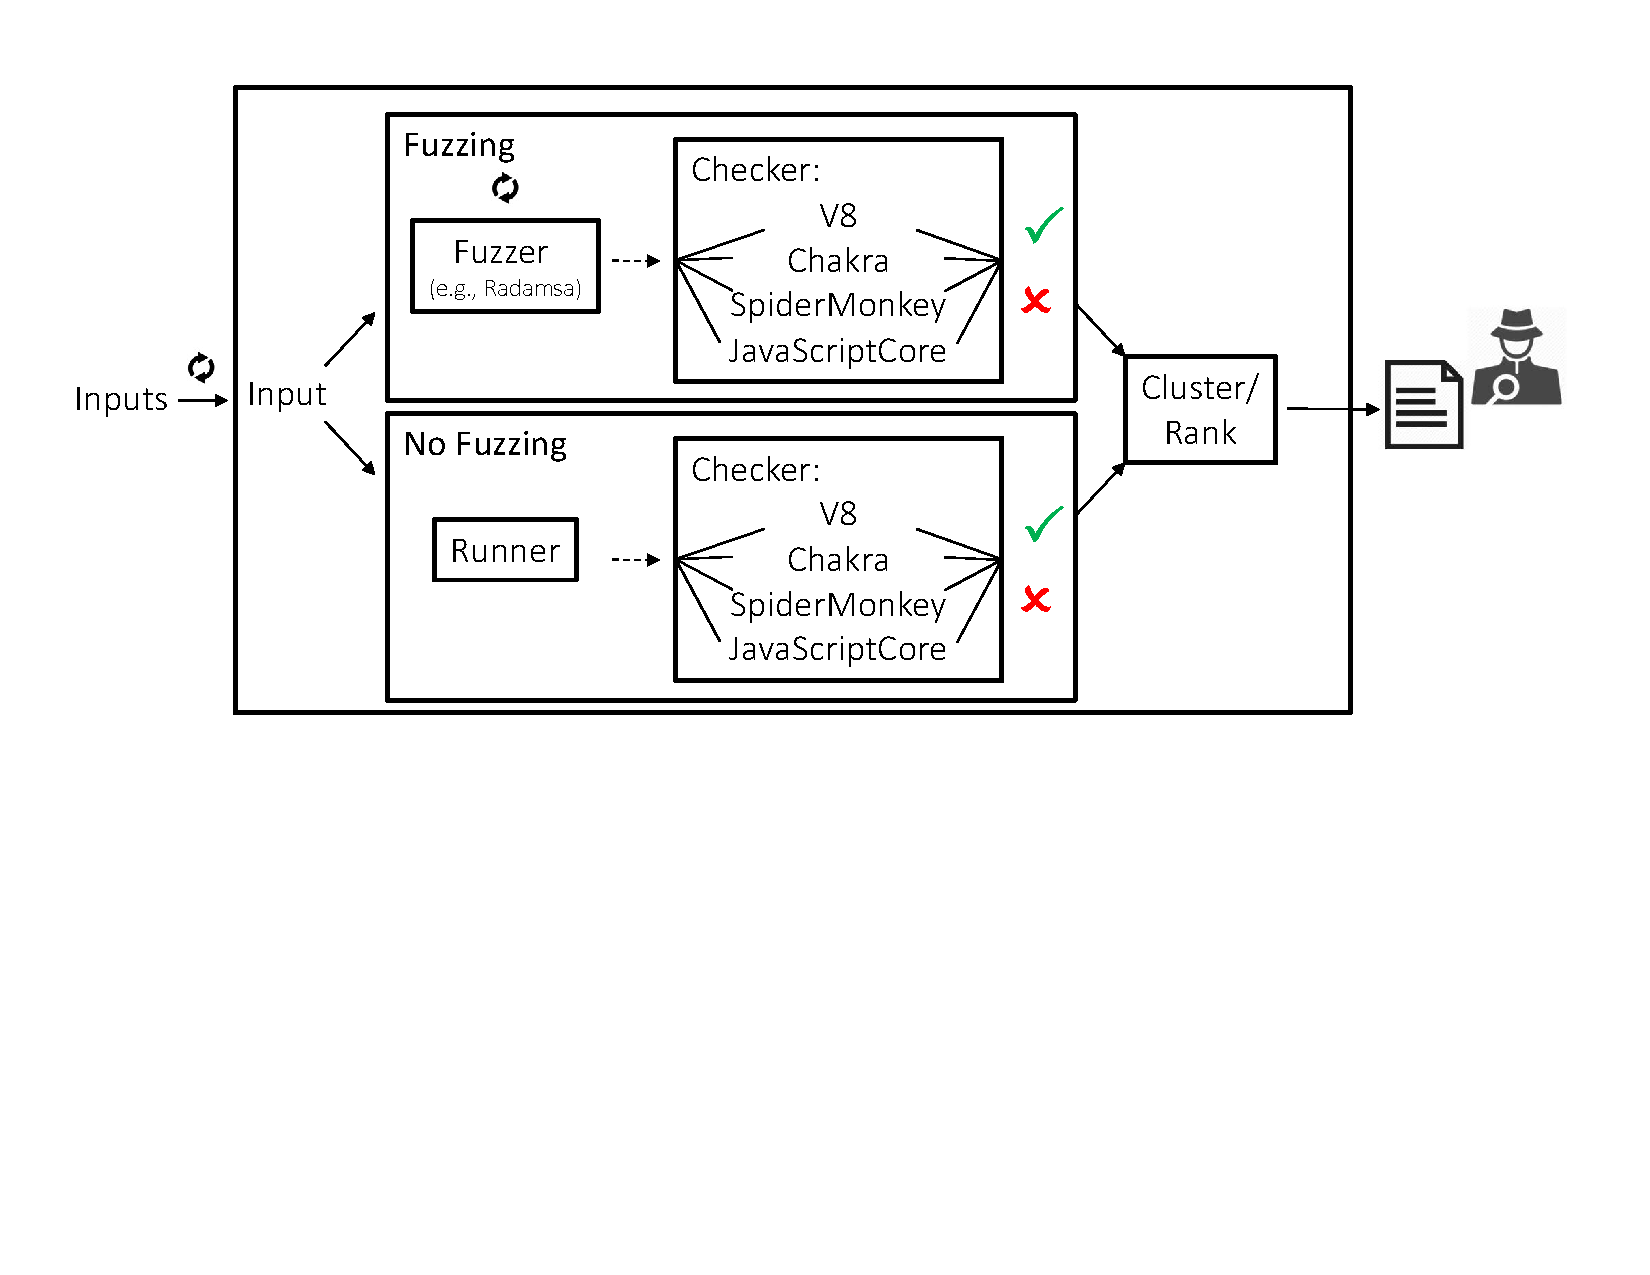
\includegraphics[trim=20 350 200
%    0,clip,width=0.35\textwidth]{google-awards-workflow}
  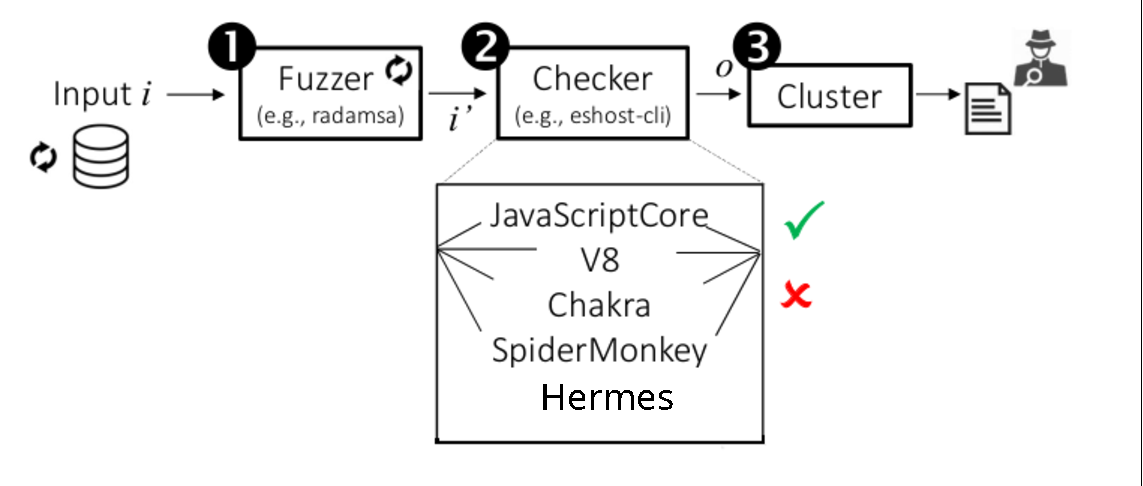
\includegraphics[trim=0 350 0 0,clip,width=0.65\textwidth]{diff-testing-runtimes}
  \caption{\label{fig:workflow}Differential Testing infrastructure overview.}
\end{figure}

Figure~\ref{fig:workflow} illustrates the infrastructure for
differential testing, which is used in part of this study. It takes on
input a list of JS files and generates warnings on output. Boxes in
the figure denote encapsulation, arrowed lines denote data flow, and
the cycle icons denote repetition--the leftmost icon indicates that
each file in the input list will be analyzed in separate whereas the
rightmost icon shows that a single file will be fuzzed multiple times.
The bug-finding process works as follows. New inputs are obtained for
a given test input using some off-the-shelf input
fuzzer~\cite{fuzz-testing-history}.\Comment{ Several fuzzing methods
  have been proposed in the past, varying with respect to how new
  inputs are
  generated~\cite{afl,honggfuzz,grammarinator,jsfunfuzz,radamsa}.}
Section~\ref{sec:objects:fuzzers} describes the fuzzers we selected.
The oracle checks whether or not the output produced for the fuzzed
file is consistent across all engines. In case the test passes in all
engines or fails in all engines (\ie{}, the output is consistent), the
infrastructure discards the test. Otherwise, it considers the input as
potentially fault-revealing; hence interesting for human
inspection. The infrastructure uses the
open-source tool eshost-cli~\cite{eshost-cli}, also used at
Microsoft, for checking output discrepancy. 

%The checker can produce multiple warnings for a given input. 

Note that a number of reasons exist, other than a bug, to explain
discrepancy (see Table~\ref{tab:false-positives}) and there is no
clear way to distinguish false and true positives automatically. As
such, a human needs to inspect the warning to classify the issue. To
facilitate inspection, we prioritized warnings and clustered them in
groups. We describe these strategies in the following.

\subsection{Prioritization}

We classified warnings in two types,
reflecting their likelihood of manifesting a real bug. Warnings of the
kind ``\hi{}'' are associated with the cases where the test code
executed to completion without violating any internal checks, but it
violated assertions declared in the test itself or its harness. The
rationale is that the input is more likely to be valid as it it did
not raise exceptions during the execution of the application code,
but, it manifested discrepancy through the violation of an assertion
declared in the test. In contrast, warnings of type ``\lo{}'' are
more likely to be asssociated with invalid inputs. They reflect the
cases where the anomaly is observed during the execution of functions,
which are part of the application. We found that different engines
often check pre-conditions of those functions differently. It can
happen, for example, that one engine enforces a weaker pre-condition
on a function input compared to another engine and that is
acceptable.\Comment{ For instance, it is acceptable to pass values greater than
\Fix{x} to function \CodeIn{\Fix{WWW}} in \Fix{y} but not in
\Fix{z}.} In those cases, the infrastructure would observe a
discrepancy that is more likely to be associated with an invalid input
produced by the fuzzer, \ie{}, it is likely to be a bug in the test
code not the engine (library or runtime) code. However, as expected, our heuristic
is not precise---``\lo'' warnings can 
reveal bugs. Figure~\ref{fig:lo-truepositive} shows one of these
cases. In this example, the test instantiates an \CodeIn{ArrayBuffer}
object and stores an 8-bit integer at the 0 position. According to the
specification~\cite{ecmas262-getviewvalue}, a \CodeIn{RangeError}
exception should be thrown if a negative value is passed to the
function \CodeIn{ToIndex}, indirectly called by the test case. In this
case, however, the \chakra{} engine did not throw any exception, which
violates the spec. This case of undocumented precondition, reported
and handled by developers as a bug, was fixed by developers after our bug
report and is no longer present in the most recent release of
\chakra. Despite that case, most bugs we found emerged from
``\hi{}'' warnings.

%% \Igor{
%%   Apesar dos bugs encontrados serem em sua maioria classificados como HI group,
%%   casos reportados como LO tambem podem ser considerados como um true positive.
%%   Nossa heuristica de classificacao eh baseada no error stream dos engenhos,
%%   se um teste falha antes da linha em que ha uma assercao, entao a falha
%%   ocorreu em uma funcao nativa do JS. Na figura \ref{fig:lo-truepositive}, \'e 
%%   possivel observar um caso de bug obtido em um bucket classificado como LO.
%%   Neste exemplo, o teste instancia um ArrayBuffer e armazena um 8-bit integer na 
%%   posicao 0 do dataframe, quando tentamos obter um elemento em uma posicao
%%   maior e/ou menor do que a suportada, neste caso \CodeIn{getInt8}, 
%%   de acordo com a especificacao\cite{ecmas262-getviewvalue}, deve-se 
%%   lancar Offset is outside the bounds.

%%   Os casos reportados no grupo LO nao foram capturados atraves das assercoes.
%%   Por exemplo, se o fuzzer gera uma entrada que viola uma especificacao, o 
%%   correto seria usar um levantar um erro
%% }

\subsection{Clusterization}
\label{sec:clusterization}

Clusterization helps to group tests that fail for similar reasons. We
only clustered ``\lo'' warnings as ``\hi'' warnings produce messages
that arise from the test case, which are typically
distinct. Figure~\ref{fig:lo-truepositive} shows, at the bottom, the
error messages produced by a ``\lo'' warning. Any warning, including
this one, that has this same message signature will be included in the
same cluster, which we may also refer as a ``bucket''.

\begin{figure}[!h]
  \centering
  \begin{lstlisting}
var buffer = new ArrayBuffer(64);
var view = new DataView(buffer);
view.setInt8(0,0x80);
assert(view.getInt8(-1770523502845470856) === -0x80);

Engines Messages (1:V8, 2:JavaScriptCore, 3:SpiderMonkey):
1. RangeError: Offset is outside the bounds of the DataView
2. RangeError: byteOffset cannot be negative
3. RangeError: invalid or out-of-range index
  \end{lstlisting}
  \caption{\label{fig:lo-truepositive}True positive example of a ``\lo''
    warning.}
\end{figure}

\section{Results}
\label{sec:results}

The goal of our study is to assess reliability of \js\ engines by
leveraging implementation diversity. We organized our study in three
parts. First, we report on the conformance of the engines we analyzed
using the official Test262 conformance test suite for
EcmaScript~\cite{ecma262-conformance-suite}
(Section~\ref{sec:stability}). In the limit, bugs would have low
relevance if the engines are too unreliable. Second, we report results
obtained with test transplantation
(Section~\ref{sec:transplantation}). The rationale is that the domain
of possible inputs is too large; consequently, we expect that test
suites written for a given engine cover scenarios and corner cases
uncovered by another engine.\Comment{ To sum, we conjecture that test
  cases written for one engine could reveal bugs in different engines
  as opposed to only manifesting false alarms.} Third, we analyzed the
impact of using cross-engine differential testing to find bugs
(Section~\ref{sec:cross-engine-diff-testing-results}). Differential
testing has been used in several contexts to address the oracle
problem~\cite{barr-etal-tse2015}. Intuitively, using differential
testing to find functional bugs across engine implementation could be
promising.

%Figure~\ref{fig:summary} summarizes the bugs we reported.

\vspace{1ex}
\noindent\textbf{Summary of Bugs.}~Figures~\ref{fig:stacked-engine}
and~\ref{fig:stacked-technique} show bugs reports per engine and
technique, respectively. Each stacked bar breaks down the bugs per
status. Note that several of these bugs were already fixed and
incorporated in the latest release of the corresponding
engines. Overall, discarding bug report with the ``new'' status, we
reported a total of \noBugsTotalConfirmed{} bugs. Considering the
engines, the majority of bug reports targeted \chakra\ and
\jsc. Considering the techniques, the number of bug reports issued
and confirmed were similar. We found, however, that the cost of
inspecting \Fix{...elaborate...}

%% It is
%% also worth noting that several of these reports hold the status
%% ``new'', which indicates that they were not reviewed yet by the
%% development team. Note also that we did not find bugs in the Mozilla
%% \smonkey\ engine.

\begin{figure}[t!]
  \centering
  \subfloat[\label{fig:stacked-engine}Bug reports per engine.]{
    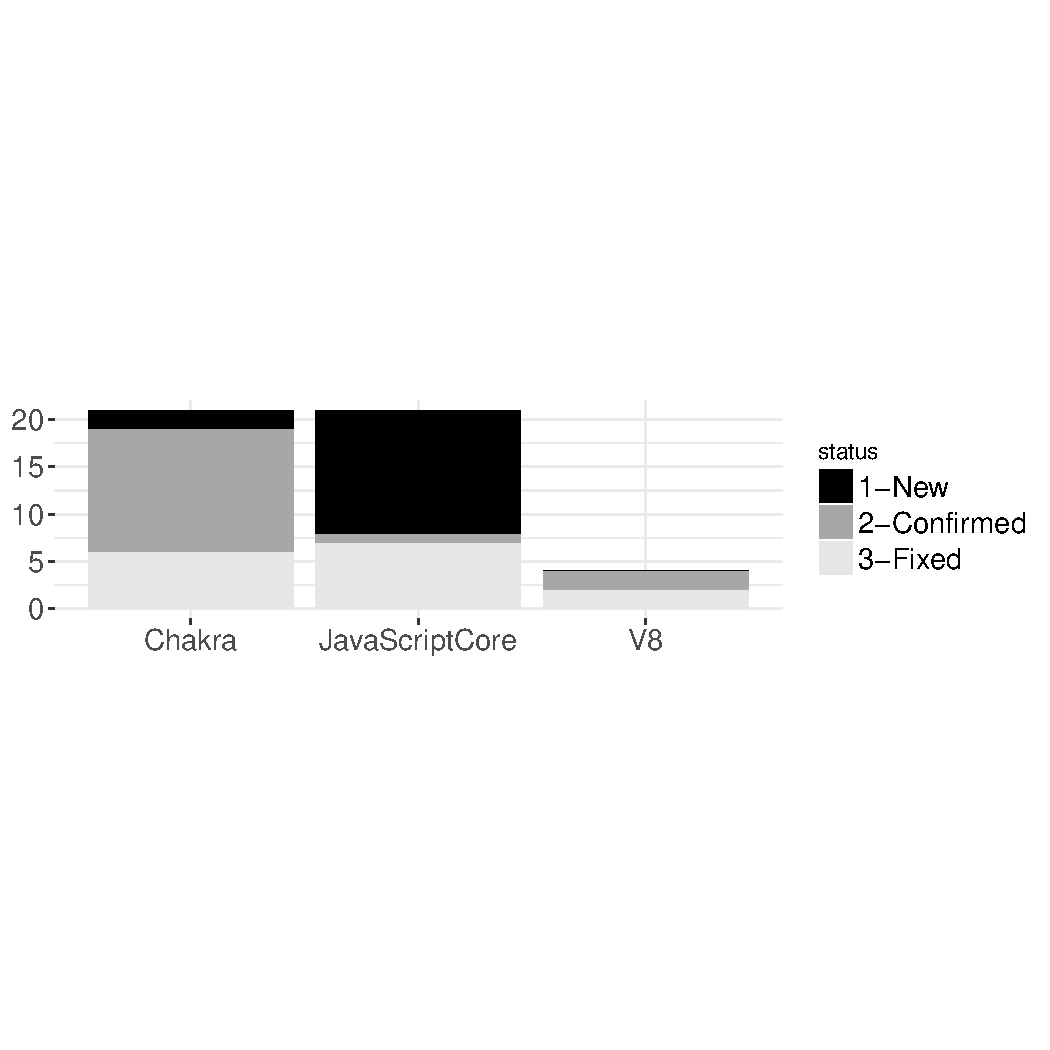
\includegraphics[trim=0 190 0 180,clip,width=0.45\textwidth,scale=0.4]{R/stackedbar/stacked-engine}
    \vspace{-5ex}
  }\\
  \subfloat[\label{fig:stacked-technique}Bugs reports per technique.]{
    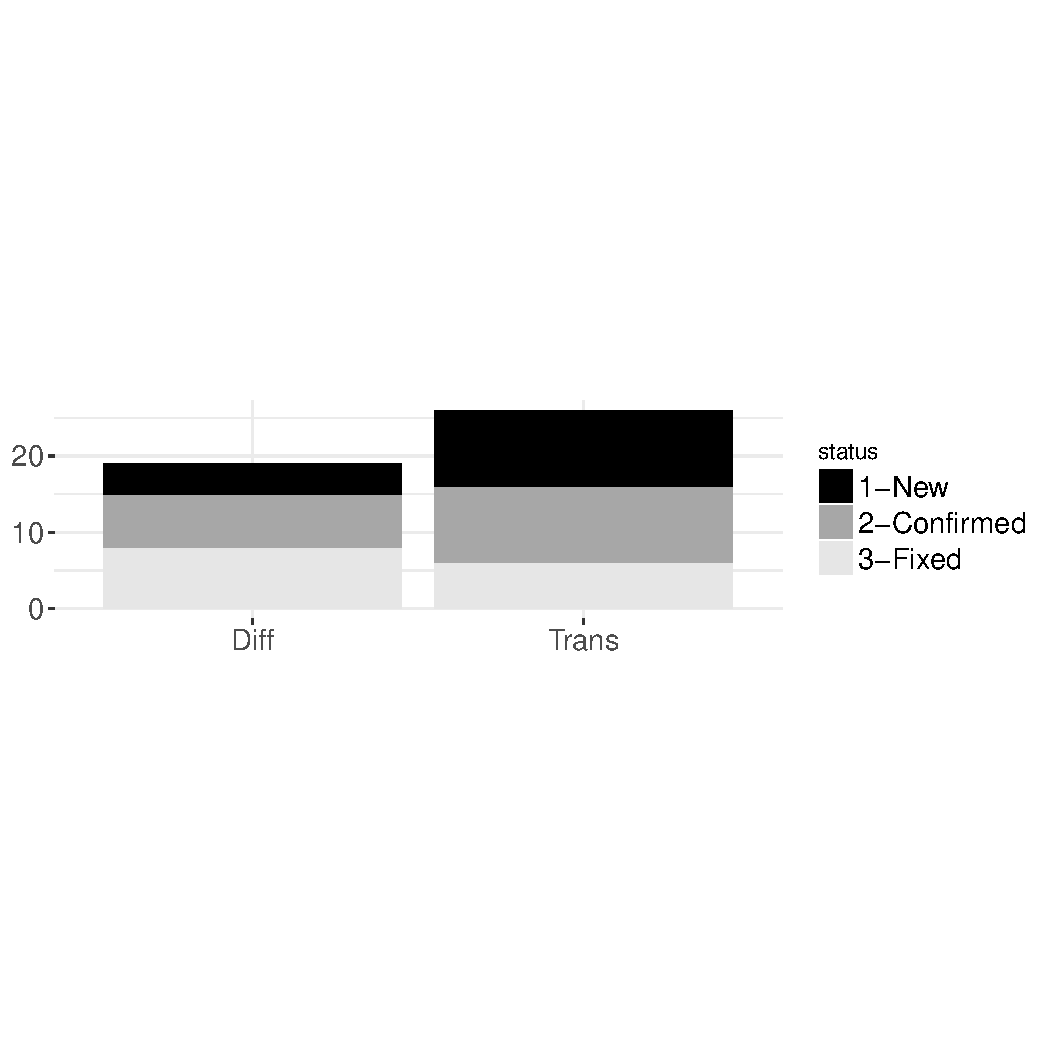
\includegraphics[trim=0 180 0 180,clip,width=0.45\textwidth,scale=0.4]{R/stackedbar/stacked-technique}
    \vspace{-5ex}        
  }
  \caption{\label{fig:summary}Summary of bug reports.}
\end{figure}

\subsection{Conformance}
\label{sec:stability}

\begin{wraptable}[12]{r}{0.25\textwidth}
  \vspace{-3ex}
  \centering
  \caption{\label{tab:test262}Percentage of passing tests on
    the Test262 conformance suite.}
  \small
  \begin{tabular}{crr}
    \toprule
    engine & \% passing \\
    \midrule
    \jsc{} & 92\%\\
    \veight{} & 95\% \\
    \chakra{} & 75\% \\    
    \smonkey{} & 93\% \\
    \bottomrule
  \end{tabular}
  \normalsize
\end{wraptable}

We used the official conformance test suite
Test262~\cite{ecma262-conformance-suite} to evaluate conformance of
engines to the \js\ current standard. As it is acceptable to release
engines fulfilling the specification only partially~\cite{kangax}, it
is expected that engines do not fully pass this test. However, we
expect that results provide indication of engine's maturity. In the
limit, it is not desirable to flood bug reports on engines at early
stages of development. We ran the suite once a day for seven
consecutive days from the period of 16 to 22 of August,
2018. Table~\ref{tab:test262} shows the average number of passing
tests over this period. The variance of results was negligible; for
that reasons, we omited standard deviations. We noticed that all four
engines we analyzed but \chakra{} use some variant of the Test262
suite as part of their regression process, but we used the same
version in this experiment; the one available from the Test262 web
site~\cite{ecma262-conformance-suite}. Results show that there are
still many unsupported cases as can be observed from the percentages
in the table, but the number of passing tests is high, with
\veight\ and \smonkey\ performing better compared to others and
\chakra\ performing well worse than others. It is important to
highlight that failures in this conformance test suite indicates
missing features as opposed to bugs. However, note that \chakra\ is
both the engine that has the lowest passing ratio in the conformance
test suite and the one we were able to find more bugs. Although it is
possible to find correlation between the percentage of passing tests
in the conformance suite (as per Table~\ref{tab:test262}) and reliability as
measured by the number of bugs found (as per
Figure~\ref{fig:summary}), we do not not imply causality.

\subsection{Test Transplantation}
\label{sec:transplantation}

This section reports results of test transplantation. More
specifically, we analyzed the failures observed when running a test
suite original from a given engine in another engine. Intuitively, we
want to assess how effective is the idea of cross-fertilization of
knowledge among \js\ developers.

\vspace{0.5ex}
\subsubsection{Methodology}
\label{sec:methodology}
In this experiment, a developer with experience in \js\ analyzed each
test file that reveals failure in a given engine and classified that
file as potentially fault-revealing or not. The co-authors supervised
the classification process to validate correctness. For the cases the
developer classified the failures as potentially fault-revealing, one
of the co-authors carefully inspected the case and reported the bug,
if confirmed, or re-classified the failure as a false alarm.

\vspace{0.5ex}
\subsubsection{Results}
\label{sec:results}

Table~\ref{tab:cross-testing} shows the number of failures observed
for each pair of test suite and engine. The first column shows the
test suites and the first row shows the engines that run those
tests. We use a dash (``-'') to indicate that we did not consider the
combinations that associate a test suite with its parent engine;
failures in those cases would either indicate regressions or flaky
tests as opposed to unknown bugs for that engine. We did not run test
cases that fail on its parent engine in any other engines; we wanted
all tests to pass on their parent engine as that would indicate that
the test case is coherent and can be used. In total, 64 test cases
were discarded for that reason--6 from \jsc{} and 57 from
\smonkey. Furthermore, we required that a test does not manifest
compile errors as we want to focus on bugs in code not in tests. For
that reason, we used the tests listed under the column
``compile-in-all'' from Table~\ref{tab:test-suites}, totalling
\totalTestFilesCompileInAll{} cases. \Mar{can you confirm that we used
  ``compile-in-all'' and not ``origina'' as these numbers
  suggest?}\Fix{In total, 7,029 test files (\ie{}, 38369-31276-64)
  were considered in this experiment, which involved 24,922 test runs
  (\ie, (7029*4)-1021-57-2116).}  Of these, 812 failures were
manifested (3.25\% of the runs) across \textbf{543} distinct files
(7.72\% of the files). We observed from
the table that, considering this dataset, the Mozilla \smonkey\ was
the engine that failed the least whereas the Microsoft engine
\chakra\ failed the most. The \smonkey\ test suite also revealed more
failures than any other, as expected, considering that it is the suite
with more tests (see Table~\ref{tab:test-suites}).

%% This suggests that the investiment in
%% testing paid off in this case.
\begin{table}[h]
  \centering
  \caption{\label{tab:cross-testing}Number of failures observed exchanging
  test suites.}
  \begin{tabular}{crrrr}
    \toprule
    test suite\textbackslash{}engine & \jsc{} & \veight{} & \smonkey{} & \chakra{}\\
    \midrule
    % \Fix{Versions (03.08)} & 234555 & 7.0.158 & 62.0b14 & 1.10.1 \\
    \Comment{
      Lembrar dos testes que os testes da propria engine falham:
      V8 0 
      JSC 2 
      Spidermonkey 58
    }
    \jsc{} & - & 9 & 10 & 58   \\
    \veight{} & 29 & - & 0 & 0  \\
%    \chakra{} & - & - & - & -  \\
    \smonkey{} & 217 & 106 & - & 278 \\
    Duktape & 0 & 4 & 4 & 1   \\
    \jerry{} & 23 & 25 & 22 & 23   \\
    JSI & 0 & 0 & 0 & 0   \\ 
   Tiny-js & 0 & 0 & 0 & 0  \\
    \midrule
   \textbf{total} & 270 & 145 & 36 & 361 \\
    \bottomrule 
  \end{tabular}
\end{table}

The sources of false positives found in this experiment are as
follows: \textbf{Undefined Behavior.} False positives of this kind are
manifested when tests cover implementation-dependent behavior, as
defined in the ECMA262 specification~\cite{ecmas262-spec}. For
example, one of the tests from \jerry\ uses the function
\CodeIn{Number.toPrecision([precision])}, which translates a number to
a string, considering a given number of significant digits. The
floating-point approximation of the real value is
implementation-dependent, making the test to pass only in \chakra\ for
that test. As another example, some tests from \Fix{Y} use the
implementation-dependent description message\Mar{what is the name of
  the property?} encapsulated in an \CodeIn{Error} object in
assertions. As such, those tests fail in all engines but
\Fix{Y}. \textbf{Timeout/OME\footnote{ome is for out of memory
    error.}.} False positives of this kind manifest because the engine
that runs the test does not optimize the code as the original engine
and that has an effect in the test outcome.  The test may fail to
finish at the specified time budget or it exceeds the memory
budget. For example, a test case from the \jsc{} suite defines a
function with a tail-call recursion. The test fails in all engines but
\jsc{}, which implements tail-call optimization, which enables the
test to finish execution fast. \textbf{Not implemented.} False
positives of this kind manifest when a test fails because it covers a
function that is part of the official spec, but is not implemented in
the target engine yet. For example, at the time of writing, \chakra{}
does not implement by default various properties from the
\mcodeid{Symbol} object. These properties are only available
activating the ES6 experimental mode with the flag
\CodeIn{-ES6Experimental}. \Mar{pela explicacao de
  ``compile-in-all'', isto nao faz sentido.$\rightarrow$} \textbf{Non-Standanrd Element.} This kind
corresponds to the cases the test case relies on some non-standard
function or property of a standard object. \Mar{revise this.$\rightarrow$}\textbf{Unknown.} This
category includes the cases we were unable to confidently diagnose the
failure but we suspected it was a false alarm.

%% \begin{figure}[h]
%%   \centering
%%   \subfloat[\label{fig:falsepositives}False Positives]{%
%%     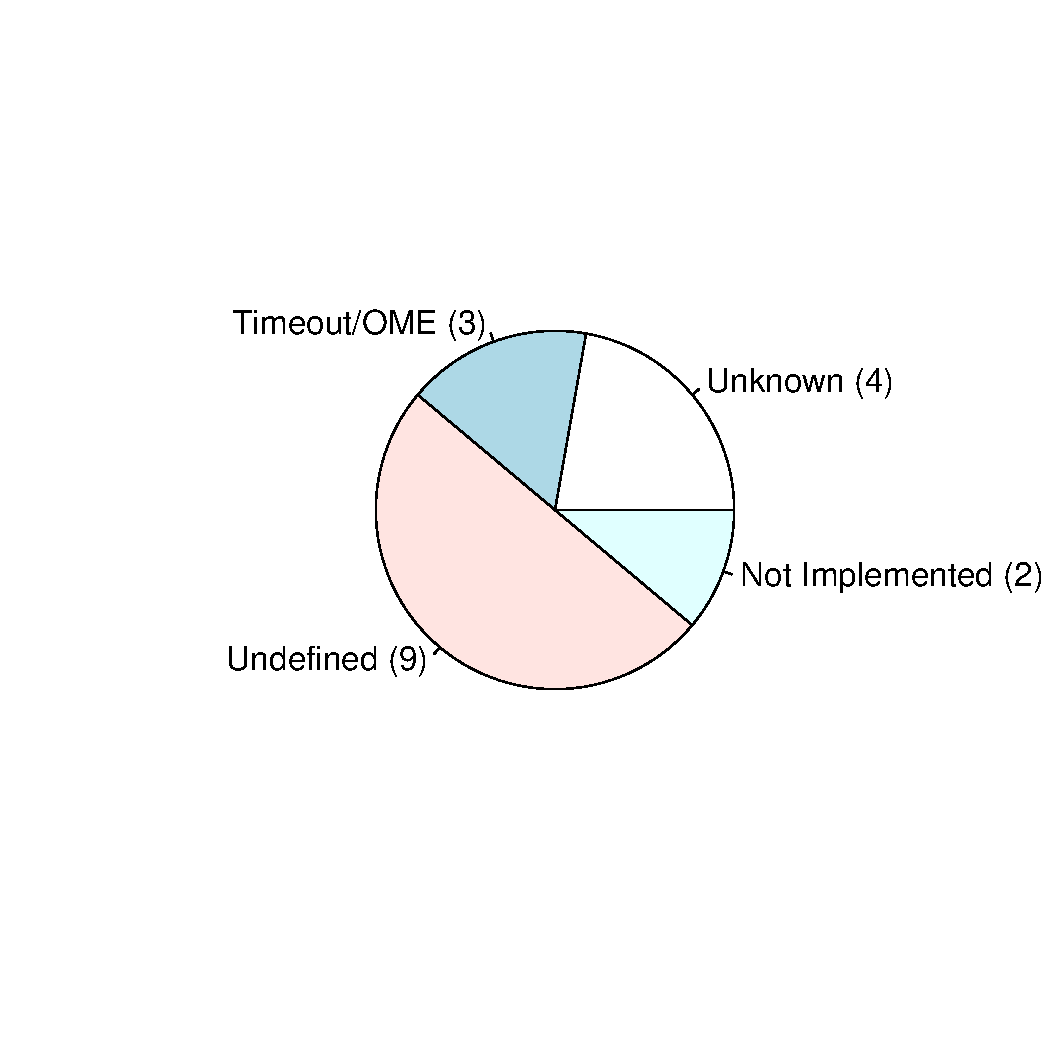
\includegraphics[trim=0 150 0 100,clip,width=0.4\textwidth]{R/piecharts/falsepositives}
%%   }
%%   \label{1a}\hfill
%%   \subfloat[\label{fig:truepositives}True Positives]{%
%%     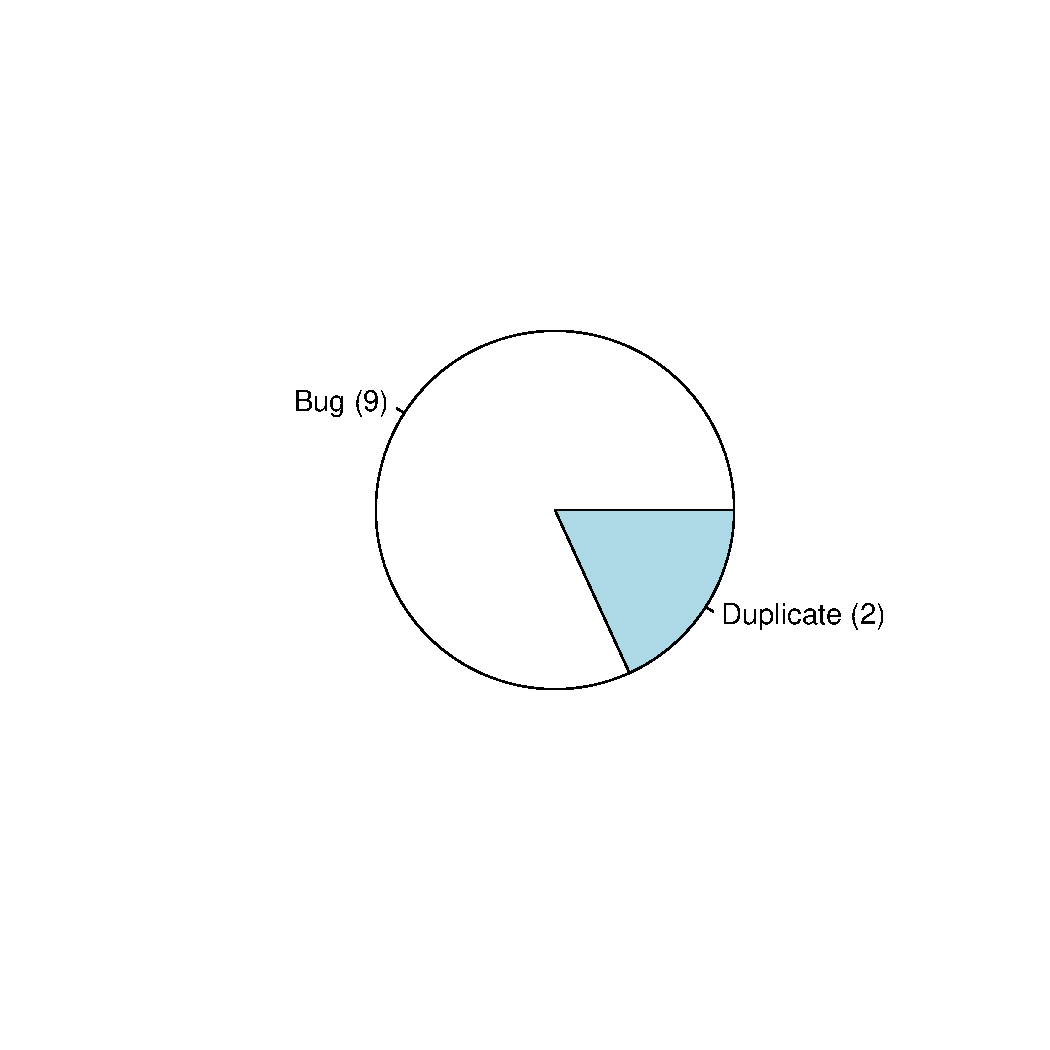
\includegraphics[trim=0 150 0 150,clip,width=0.4\textwidth]{R/piecharts/truepositives}    
%%   }
%%   \label{1b}\\
%%   \caption{\label{fig:piecharts-transplantation}False and True positives.}
%% \end{figure}

\begin{table}[h!]
  \setlength{\tabcolsep}{4pt}    
  \centering
  \caption{\label{fig:falsepositives}\label{fig:truepositives}\label{fig:piecharts-transplantation}Distribution of false and true positives.}
  \begin{tabular}{ccr}
    \toprule
    & source &  \#\\
    \midrule
    \multirow{5}{*}{False Positives} & Undefined Behavior & 313 \\
    & Timeout/OME & 13 \\
    & Not Implemented & 21 \\
    & Non-Standard Element & \Fix{132} \\
    & Unknown & \Fix{-} \\
    \midrule
    \multirow{2}{*}{True Positives} & Duplicate & 9 \\
    & Bug & 24 \\
    \bottomrule
  \end{tabular}
\end{table}

%%  The piechart at the top
%% shows false alarms. The absolute number of tests in each category is
%% shown in parentheses to the right-side of each slice label naming the
%% source of false positive.  


\begin{table}[t!]
  %\small
%  \setlength{\tabcolsep}{5pt}
  \renewcommand{\arraystretch}{0.9}
  %  \vspace{-3ex}
    %  \scriptsize
      \centering
      \caption{List of bugs reports from Test Transplantation.}
      \label{tab:test-transplantation-bugs}

      \begin{tabular}{rccccc}

        \toprule \# & Engine  & Version & Status & Severity & Suite \\
        \midrule
       1  & \jsc{} & 606.1.9.4 & New  & - & \jerry{} \\
       2  & \chakra{}  & 1.9 & \textbf{Confirmed} & 2 & \smonkey{} \\
       3  & \chakra{}  & 1.9 & \textbf{Fixed}   & 2 & \smonkey{} \\
%      \midrule
       4  & \chakra{} & 1.10-beta & \textbf{Confirmed} & 2 & \smonkey{} \\
       5  & \jsc{} & 606.1.9.4 & New &  -  & \smonkey{}\\
%      \midrule
       6  & \jsc{} & 606.1.9.4 & New & - & \smonkey{} \\
       7  & \jsc{} & 606.1.9.4 & \textbf{Fixed} & 2 & \smonkey{}\\ % webkit
       8  & \chakra{} & 1.10-beta & \textbf{Fixed} & 3 & \smonkey{}\\
       9  & \chakra{} & 1.10-beta & \textbf{Fixed} & 2 & \jsc{}\\
       10 & \chakra{} & 1.10-beta & \textbf{Fixed} & 2 & \smonkey{}\\
       11 & \chakra{} & 1.11-beta & \textbf{Fixed} & 2 & \jsc{}\\
       12 & \chakra{} & 1.11-beta & \textbf{Confirmed} & 2 & \jerry{}\\ % duktape
       13 & \chakra{} & 1.10.1 & \textbf{Fixed} & 2 & \smonkey{}\\
       14 & \jsc{} & 233840 & Duplicated & 2 & \jerry{}\\
       15 & \chakra{} & 1.10.1 & \textbf{Fixed} & 2 & \jerry{}\\ % test262
       16 & \chakra{} & 1.10.1 & \textbf{Fixed} & 3 & \jerry{}\\
       17 & \jsc{} & 234555 &\textbf{Fixed} & 2 & \jerry{}\\
       18 & \chakra{} & 1.10.1 & \textbf{Fixed} & 3 & \jerry{}\\
       19 & \jsc{} & 234654 & \textbf{Fixed} & 2 & \jerry{}\\
       20 & \veight{} & 7.0.181 & \textbf{Fixed} & 3 & \jerry{}\\
       21 & \jsc{} & 234689 & New & - & \jerry{}\\
       22 & \veight{} & 7.0.237 & WontFix & 2 & Duktape\\
       23 & \chakra{} & 1.10.2 & \textbf{Fixed} & 2 & \smonkey{}\\
       24 & \jsc{} & 235121 & \textbf{Fixed} & 2 & \smonkey{}\\
       25 & \jsc{} & 235121 & \textbf{Fixed} & 2 & \smonkey{}\\
       26 & \veight{} & 7.0.244 & \textbf{Fixed} &  2  & \smonkey{}\\
       27 & \chakra{} & 1.10.2 & \textbf{Fixed} &  2  & \smonkey{}\\
       28 & \jsc{} & 235121 & New & - & \smonkey{}\\
       29 & \chakra & 1.11.19 & \textbf{Confirmed}  & - & \babel \\
       30 & \jsc & 262693 & New & - & \babel \\
       31 & \jsc    & 262693 & New & - & \babel \\
       32 & \smonkey & 77.0b9 & \textbf{Fixed} & 3 & \hermes\\
       %33 & \hermes & 0.5.0 & WontFix & - & \babel \\
       %34 & \hermes & 0.5.0 & \textbf{Confirmed} & - & \babel \\
       %35 & \hermes & 0.5.0 & WontFix  & - & \babel \\
       \bottomrule
      \end{tabular}
      \vspace{-2ex}
\end{table}

% JavaScript-C77.0 (77.0b9)
% tracking urls
% 1  & 4/18  & \jsc{} & 606.1.9.4 & New  & \href{https://bugs.webkit.org/show\_bug.cgi?id=184749}{\#184749} & - & \jerry{} \\
% 2  & 4/23 & \chakra{}  & 1.9 & \textbf{Confirmed}  & \href{\repoCH/issues/5033}{\#5033} & 2 & \smonkey{} \\
% 3  & 4/29 & \chakra{}  & 1.9 & \textbf{Fixed}   & \href{\repoCH/issues/5065}{\#5065} & 2 & \smonkey{} \\
% 4  & \multirow{2}{*}{4/29} & \chakra{} & 1.10-beta & \textbf{Confirmed} & \href{\repoCH/issues/5067}{\#5067} & 2 & \smonkey{} \\
% 5  &  & \jsc{} & 606.1.9.4 & New & \href{https://bugs.webkit.org/show\_bug.cgi?id=185130}{\#185130} &  -  & \smonkey{}\\
% 6 & 5/02  & \jsc{} & 606.1.9.4 & New  & \href{https://bugs.webkit.org/show\_bug.cgi?id=185208}{\#185208} & - & \smonkey{} \\
% 7 & \multirow{2}{*}{5/02}  & \jsc{} & 606.1.9.4 & \textbf{Fixed} & \href{https://bugs.webkit.org/show_bug.cgi?id=185211}{\#185211} & 2 & \smonkey{}\\ % webkit
% 8 &  & \chakra{} & 1.10-beta & \textbf{Fixed} & \href{\repoCH/issues/5087}{\#5087} & 3 & \smonkey{}\\
% 9 & 5/17  & \chakra{} & 1.10-beta & \textbf{Fixed} & \href{\repoCH/issues/5187}{\#5187} & 2 & \jsc{}\\
% 10 & 5/21  & \chakra{} & 1.10-beta & \textbf{Fixed} & \href{\repoCH/issues/5203}{\#5203} & 2 & \smonkey{}\\
% 11 & 6/28  & \chakra{} & 1.11-beta & \textbf{Fixed}  & \href{\repoCH/issues/5388}{\#5388} & 2 & \jsc{}\\
% 12 & 7/10  & \chakra{} & 1.11-beta & \textbf{Confirmed} & \href{\repoCH/issues/5442}{\#5442} & 2 & \jerry{}\\ % duktape
% 13 & 7/18  & \chakra{} & 1.10.1 & \textbf{Fixed} & \href{\repoCH/issues/5478}{\#5478} & 2 & \smonkey{}\\
% 14 & 7/18  & \jsc{} & 233840 & Duplicated & \href{https://bugs.webkit.org/show_bug.cgi?id=187777}{\#187777} & 2 & \jerry{}\\
% 15 & 7/18  & \chakra{} & 1.10.1 & \textbf{Fixed} & \href{\repoCH/issues/5549}{\#5549} & 2 & \jerry{}\\ % test262
% 16 & 8/07  & \chakra{} & 1.10.1 & \textbf{Fixed} & \href{\repoCH/issues/5576}{\#5576} & 3 & \jerry{}\\
% 17 & 8/07  & \jsc{} & 234555 &\textbf{Fixed} & \href{https://bugs.webkit.org/show_bug.cgi?id=188378}{\#188378} & 2 & \jerry{}\\
% 18 & 8/07  & \chakra{} & 1.10.1 & \textbf{Fixed} & \href{\repoCH/issues/5579}{\#5579} & 3 & \jerry{}\\
% 19 & 8/07  & \jsc{} & 234654 & \textbf{Fixed} & \href{https://bugs.webkit.org/show_bug.cgi?id=188382}{\#188382} & 2 & \jerry{}\\
% 20 & 8/08  & \veight{} & 7.0.181 & \textbf{Fixed} & \href{https://bugs.chromium.org/p/v8/issues/detail?id=8033}{\#8033} & 3 & \jerry{}\\
% 21 & 8/08  & \jsc{} & 234689 & New & \href{https://bugs.webkit.org/show_bug.cgi?id=188407}{\#188407} & - & \jerry{}\\
% 22 & 8/16  & \veight{} & 7.0.237 & WontFix & \href{https://bugs.chromium.org/p/v8/issues/detail?id=8064}{\#8064} & 2 & Duktape\\
% 23 & 8/22  & \chakra{} & 1.10.2 & \textbf{Fixed} & \href{\repoCH/issues/5621}{\#5621} & 2 & \smonkey{}\\
% 24 & 8/22  & \jsc{} & 235121 & \textbf{Fixed} & \href{https://bugs.webkit.org/show_bug.cgi?id=188874}{\#188874} & 2 & \smonkey{}\\
% 25 & \multirow{3}{*}{8/22} & \jsc{} & 235121 & \textbf{Fixed} & \href{https://bugs.webkit.org/show_bug.cgi?id=188875}{\#188875} & 2 & \smonkey{}\\
% 26 &  & \veight{} & 7.0.244 & \textbf{Fixed} & \href{https://bugs.chromium.org/p/v8/issues/detail?id=8082}{\#8082} &  2  & \smonkey{}\\
% 27 &  & \chakra{} & 1.10.2 & \textbf{Fixed} & \href{\repoCH/issues/5624}{\#5624} &  2  & \smonkey{}\\
% 28 & 8/23  & \jsc{} & 235121 & New & \href{https://bugs.webkit.org/show_bug.cgi?id=188877}{\#188877} & - & \smonkey{}\\


Table~\ref{fig:piecharts-transplantation} shows the distribution of
false and true positives. Considering false positives, ``Undefined
Behavior'' and ``Non-Standard Element'' were the most predominant
sources. Considering true positives, we found a reasonable number of
duplicate reports, but not enough high to justify attempting to
automate the detection of duplicates.
Table~\ref{tab:test-transplantation-bugs} lists all bugs we found with
test transplantation. The first column shows the identifier we
assigned to the bug\Comment{, column ``Date'' shows the date the bug
  was reported in the format ``m/dd'',} column ``Engine'' shows the
affected engine, column ``Status'' indicates the status of the bug
report at the time of the writing (\eg{},``New'', ``Rejected'',
``Confirmed'', ``Fixed''). The status string appear in bold face for
status ``Confirmed'' or higher (\ie{}, ``Assigned'' or ``Fixed'').
Column ``Url'' shows the URL (de-anonymized upon request) for the bug report entry in the
corresponding bug-tracking system, column ``Severity''
shows the severity level for confirmed bugs, and, finally, column
``Suite'' shows the name of the engine that originated the
test. Note that bug reports \#4 and \#23 afected multiple engines.

Considering severity levels, it is important to note that \jsc{}
uses five levels~\cite{jsc-severity} whereas
\chakra{}~\cite{chakra-severity} and
\smonkey{}~\cite{mozilla-severity} use only two. As usual, the
smallest the severity value the highest the severity of the bug. We
use a dash (``-'') as the severity level for bugs with pending
confirmation.  No bug we reported in this experiment was rejected.  Of
the \Fix{17} bugs we reported in this experiment, \Fix{9} were
analyzed and moved from the status ``New'' to ``Confirmed''. Of these,
\Fix{8} are severity-2 bugs.  Although we did not find any showstopper
critical bugs, most of the bugs are seemingly important as per the
categorization given by engineers. Analyzing the issue tracker of
\chakra, we found that severity-1 bugs are rare. Considering the bugs
confirmed by developers, \chakra{} was the engine with the highest
number, \Fix{8} in total, with \Fix{1} bug fixed. Considering the
remaining engines, \veight{} developers confirmed \Fix{one} bug we
reported. Curiously, Google engineers confirmed that report in a few
hours. We found that development teams of other engines, specially
\jsc\, took much longer to analyze bug reports as can be observed by
some pending reports from April 2018.

Overall, we found these results promising given that precision (\ie{},
the ratio of true positives over all reports) needs to take into
account the cost of inspecting the failure~\cite{harman-ohearn-2018};
it took a week for the developer to inspect the entire set of
failures. The precision for \jsc\ was \Fix{X\%} (\ie, XX/270), which
seems a low rate, but it took approximately \Fix{x} days to find
\Fix{y} real bugs on this engine. Section~\ref{sec:bugs} shows samples
of false and true positives.

\begin{center}
  \fbox{
    \begin{minipage}{8cm}
      \textit{Summary:}~Test transplantation is effective at finding
      functional bugs. Although the inspection cost is non-negligible,
      the approach was able to reveal several bugs in widely popular
      engines.
      \end{minipage}
    }
\end{center}



\subsection{Cross-Engine Differential Testing}
\label{sec:cross-engine-diff-testing-results}

This section reports the results obtained with differential
testing. More precisely, we report results obtained by fuzzing test
inputs, running those inputs on different engines, and checking the
outcomes with a differential oracle.  We configured our infrastructure
(see Figure~\ref{fig:workflow}) to produce 20 well-formed fuzzed files
per input file, \ie{}, the number of fuzzing iterations can exceed the
number above as we discard syntactically invalid files.

\vspace{0.5ex}
\subsubsection{Methodology}
The methodology we used to assess effectiveness of this technique is
as follows. To avoid experimental noise, we only fuzz test files that
pass in all engines.  This corresponds to the tests appearing under
the column ``no-fail-in-all'' from Table~\ref{tab:test-suites}--a
total of \totalTestFilesPassInAll\ tests satisfy this restriction.
The intuition is that we wanted to avoid the scenario where fuzzing
produces a fault-revealing input based on a test that was already
revealing failures on some engine. This decision ensures that we can
establish cause-effect relationship between fuzzing and the
observation of discrepancy. 

\vspace{0.5ex}
\noindent\textbf{Exploratory Phase.} For the first three months of the
study, our inspection process was exploratory.  In this phase, we
wanted to learn whether or not black-box fuzzers could reveal real
bugs and how effective \lo\ warnings were relative to
\hi\ warnings. Considering the choice of fuzzers, we did find several
bugs with \radamsa\, but only some with \quickfuzz. The rationale for
studying the the \hi\ and \lo\ warning classification was that if we
found that the ratio of bugs from \lo\ warnings was rather low, we
could focus our inspection efforts only on \hi\ warnings as we
expected the number of warnings to increase dramatically compared to
the previous experiment. That finding would be important to reduce
inspection cost and guide future developments of this approach. To run
this experiment, we trained eight students in analyzing the warnings
that our infrastructure produces. The students were enrolled in a
graduate-level testing class. We listed warnings in a spreadsheet and
requested the students to update an ``owner'' column indicating who
was working on it, but we did not enforce a strict order on the
warnings the students should inspect. Recall from
Section~\ref{sec:clusterization} that we clustered \lo\ warnings in
buckets. For that reason, we only listed one \lo\ warning per
representative class/bucket in the spreadsheet. First, we explained,
through examples, the possible sources of false alarms they could find
and then we asked the students to use the following procedure when
finding a suspicious warning. Analyze the parts of the spec related to
the problem and, if still suspicious, look for potential duplicates on
the bug tracker of the affected engine using related keywords. If none
was reported, indicate in the spreadsheet that that warning is
potentially fault-revealing. We encouraged students to use
lithium~\cite{lithium} to minimize long test cases; the tests from the
Mozilla suite are often longer than others. Only after the co-authors
checked the potential bugs, a bug report was filed. Each student found
at least one bug using this methodology.

\vspace{0.5ex}
\noindent\textbf{Non-Exploratory Phase.} Results obtained in the
exploratory phase confirmed our expectations that most of the bugs
found during the initial three months of investigation were related to
\hi\ warnings. For that reason, we changed our inspection
strategy. This time, only the co-authors inspected the bugs using a
similar discipline as before. However, the set of warnings inspected
and the order of inspection changed. We restricted our analysis to
\hi\ warnings and, aware that we would be unable to analyze each and
every warning reported, we grouped those warnings per engine,
analyzing each group in a round-robin fashion.  At each iteration, we
analyzed \Fix{five} warnings in each group. A warning belongs to the
group of a given engine if only that engine manifests distinct
behavior, \ie{}, it produces a distinct output compared to others. We
separated in a distinct group the warnings for which two engines
diverge. The rationale for this methodology was to give attention to
each engine more uniformly, enabling more fair comparison across
engines.

\vspace{0.5ex}
\subsubsection{Results} In this section we discuss results obtained
across these two phases of the experiment. Table~\ref{tab:summary-lo}
shows statistics of \lo\ warnings obtained when fuzzing inputs with
different tools. Column ``\# buckets'' shows the number of buckets
associated with ``\lo'' warnings, column ``\# files'' shows the total
number of files involved in these warnings, and column ``avg. \# files
per bucket'' show the average number of files per bucket. Note that,
although the number of buckets and files differ substantially across
fuzzers, the difference of files per bucket was negligible.

\begin{table}[h]
  \centering
  \caption{\label{tab:summary-lo}Summary of \lo\ warning reports.}
  \begin{tabular}{crrr}
    \toprule
    & \# buckets & \# files & avg. \# files per bucket \\
    \midrule
    \radamsa{} & 82 & 241 & 2.9 \\
    \quickfuzz{} & 38 & 87 & 2.3 \\
    \bottomrule
  \end{tabular}
\end{table}

Table~\ref{tab:summary-hi} shows statistics of \hi\ warnings; recall
from Section~\ref{sec:clusterization} that we do not cluster
\hi\ warnings\Comment{ as there was no clear clustering criteria to
  use for that}. This table breaks down \hi\ warning by the affected
engine, \ie, the engine manifesting distinct output among those
analyzed. Column ``+1'' show the cases where more than one engine
disagree on the output. Note that the ordering of engines considering
this metric is consistent with the one observed on
Table~\ref{tab:cross-testing}, with \chakra\ and \jsc\ holding first
and second place, respectively, in number of warnings (resp.,
failures) compared to other engines.
%\veight\ and \smonkey. 

\begin{table}[h]
  \setlength{\tabcolsep}{5pt}
  \centering
  \caption{\label{tab:summary-hi}Number of \hi\ warning
    reports per engine.\Fix{falta add test262}}
  \begin{tabular}{crrrrr}
    \toprule
    fuzzer\textbackslash{}engine & \jsc\ & \veight\ & \chakra & \smonkey & +1\\
    \midrule
    \radamsa{} & 30 & 4 & 121 & 3 & 143 \\
    \quickfuzz{} & 12 & 7 & 67 & 8 & 89 \\
    \bottomrule
  \end{tabular}
\end{table}

Table~\ref{tab:false-positives} shows the distribution of false
positives per source. The sources of imprecision are as defined in
Section~\ref{sec:transplantation} with the addition of three new
sources, which we did not observe before. These sources are
highlighted with a ``*'' in the table. The source ``Invalid Input''
indicates that the test input violated some part of the
specification. For example, the test indirectly invoked some function
with unexpected arguments; this happens because fuzzing is not
sensitive to function specifications.

%% \Igor{devemos remover isso da 
%% etapa de fuzzing upcoming feature falha mesmo sem fuzzing...$\rightarrow$
%% The source ``Upcoming Feature''
%% indicates that the test fails because it uses a feature that is
%% available in the original engine, but it is still not standard, and
%% the target engine does not support that feature}. For example,
%% \Fix{provide concrete example}. \Fix{explain error message mismatch}

\begin{table}[h]
  \centering
  \caption{\label{tab:false-positives}Distribution of false
    and true positives.}
  \begin{tabular}{ccrr}
    \toprule
    & & \radamsa\ & \quickfuzz\ \\
    \midrule
    \multirow{5}{*}{False Positives} & Undefined Behavior & 18 & - \\
    & Timeout/OME & 23 & - \\
    & Not Implemented & 19 & - \\
    & * Invalid Input & 10 & - \\    
    & * Error Message Mismatch & 3 & - \\
    \midrule
    \multirow{2}{*}{True Positives} & Duplicate & - \\
    & Bug & - \\
    \bottomrule     
  \end{tabular}
\end{table}

Table~\ref{tab:bugs} shows the list of bugs we reported. The table is
organized in two sections. The top section shows results obtained
during the exploratory phase of the study and the bottom section shows
the results obtained during the non-exploratory phase. The table shows
the date the bug was reported (``Date''), the fuzzing tool used
(``Fuzz''), the \js\ engine affected (``Engine''), the status of the
bug report as of Aug. 24, 2018 (``Status''), the Url of the bug report
(``Url''), the severity of the bug report (``Severity''), the priority
that we assigned to the warning that revealed the bug (``Priority''),
and the test suite from the original test input (``Suite'').

So far, ten of the bugs we reported were confirmed, two of
which were fixed. One bug report we submitted was rejected on the
basis that the offending JS file manifested an incompatibility across
engine implementations that was expected.  Note from the table that
all bug reports still waiting for confirmation are associated with the
\jsc{} engine. A closer look at the \jsc{} issue tracker showed that
their triage process is slow relative to \chakra's.\Comment{\Igor{ The bugs
  reported on \chakra{}'s bug tracker was defined as confirmed,
  however the bugs are included on a milestone for the next release
  following an internal priority.  }} As of now, we did not find any
new bug on \smonkey{} and V8; the bugs we found were duplicates and
were not reported.

%% Finally, it is worth noting that \Fix{11 of the 19}
%% JS files that manifested discrepancies were \emph{not} produced with
%% fuzzing (column ``Fuzz''). These are test files from suites of
%% different engines. This observation emphasizes the importance of
%% continuously collecting test suites from multiple sources; today, we
%% use test suites from seven different open source engines, including a
%% total of 30K test files.

\begin{table*}[h!]
  \vspace{-3ex}
%  \scriptsize
  \centering
  \caption{List of bug reports issued as result of cross-engine
    differential testing.}
  \label{tab:bugs}
  \begin{tabular}{ccccccccc}
    \toprule
    Issue\#    & Date & Fuzz & Engine  & Status  &
    \multicolumn{1}{c}{Url}  & Severity & Priority & Suite \\
    \midrule
%    \multicolumn{9}{c}{\emph{Exploratory Phase}} \\
%    \midrule    
    1  & 4/12 & radamsa & \chakra{}   & \textbf{Fixed}  &
    \anonym{\href{https://github.com/Microsoft/\chakra{}Core/issues/4978}{\#4978}}
    & 2 & \textbf{\lo} & \jsc{} \\ 
    2  & 4/12 & radamsa & \chakra{}   & Rejected  &
    \anonym{\href{https://github.com/Microsoft/\chakra{}Core/issues/4979}{\#4979}}
    & - & \hi{} & \jsc{} \\
    3  & 4/14 & radamsa & \jsc{}  & New &
    \anonym{\href{https://bugs.webkit.org/show\_bug.cgi?id=184629}{\#184629}
    } & -  & \hi{} & \jsc{}    \\
    4  & 4/25 & radamsa & \chakra{}  & \textbf{Fixed}     &
    \anonym{\href{https://github.com/Microsoft/\chakra{}Core/issues/5038}{\#5038}}
    & 2 & \hi{} & \jerry{}   \\
    5  & 4/29 & radamsa & \jsc{}  & \textbf{Fixed}  &
    \anonym{\href{https://bugs.webkit.org/show\_bug.cgi?id=185127}{\#185127}
    } & 2  & \hi{}  & \jerry{}\\
    
    \midrule
    \multirow{2}{*}{6} & \multirow{2}{*}{4/30}  &
    \multirow{2}{*}{radamsa} & \chakra{} & \textbf{Confirmed} &
    \anonym{\href{https://github.com/Microsoft/\chakra{}Core/issues/5076}{\#5076}}
    & 2 & \multirow{2}{*}{\hi{}} & \multirow{2}{*}{TinyJS}\\    
                        &                        &        &
    \jsc{} & New &
    \anonym{\href{https://bugs.webkit.org/show\_bug.cgi?id=185156}{\#185156}}
    & - &  & \\
    \midrule

    
    7 & 5/02 & radamsa & \jsc{}  & \textbf{Fixed} &
    \anonym{\href{https://bugs.webkit.org/show\_bug.cgi?id=185197}{\#185197}}
    & 2 & \textbf{\lo} & \smonkey{} \\
    8 & 5/10 & radamsa & \chakra{} & \textbf{Confirmed} &
    \anonym{\href{https://github.com/Microsoft/\chakra{}Core/issues/5128}{\#5128}}
    & 3 & \hi{} & \jerry{} \\
    9 & 5/17 & radamsa & \chakra{} & \textbf{Fixed} &
    \anonym{\href{https://github.com/Microsoft/\chakra{}Core/issues/5182}{\#5182}}
    & 2 & \hi{} & \veight{}\\
    10 & 5/24 & radamsa & \jsc{} & \textbf{Fixed}  &
    \anonym{\href{https://bugs.webkit.org/show\_bug.cgi?id=185943}{\#185943}}
    & 2 & \hi{} & \jsc{}\\
    11 & 6/26 & radamsa & \jsc{} & \textbf{Fixed}  &
    \anonym{\href{https://bugs.webkit.org/show_bug.cgi?id=187042}{\#187042}}
    & 2 & \hi{} & \jerry{}\\
    12 & 7/10 & quickfuzz & \jsc{} & \textbf{Fixed}  &
    \anonym{\href{https://bugs.webkit.org/show_bug.cgi?id=187520}{\#187520}}
    & 2 & \hi{} & \jerry{}\\
    13 & 7/10 & quickfuzz & \chakra{} & \textbf{Confirmed}  &
    \anonym{\href{https://github.com/Microsoft/\chakra{}Core/issues/5443}{\#5443}}
    & 2 & \hi{} & \jerry{}\\
    %    \multicolumn{9}{c}{\emph{Non-Exploratory Phase}} \\

    \midrule
    \multirow{2}{*}{14} & \multirow{2}{*}{8/21}  &
    \multirow{2}{*}{radamsa} & \chakra{} & \textbf{Confirmed} &
    \anonym{\href{https://github.com/Microsoft/\chakra{}Core/issues/5617}{\#5617}}
    & - & \multirow{2}{*}{\hi{}} & \multirow{2}{*}{Test262}\\    
    & & &
    \veight{} & \textbf{Fixed} &
    \anonym{\href{https://bugs.chromium.org/p/v8/issues/detail?id=8078}{\#8078}}
    & 2 &  & \\
    \midrule
    
    15 & 8/23 & quickfuzz & \jsc{} & New  &
    \anonym{\href{https://bugs.webkit.org/show_bug.cgi?id=188899}{\#188899}}
    & - & \hi{} & Test262\\
    16 & 8/23 & quickfuzz & \veight{} & \textbf{Confirmed}  &
    \anonym{\href{https://bugs.chromium.org/p/v8/issues/detail?id=8088}{\#8088}}
    & 2 & \hi{} & Test262\\

    \midrule
    \multirow{2}{*}{17} & \multirow{2}{*}{8/24}  &
    \multirow{2}{*}{quickfuzz} & \chakra{} & New &
    \anonym{\href{https://github.com/Microsoft/\chakra{}Core/issues/5630}{\#5630}}
    & - & \multirow{2}{*}{\hi{}} & \multirow{2}{*}{Test262}\\    
    & & & 
    \jsc{} & New &
    \anonym{\href{https://bugs.webkit.org/show_bug.cgi?id=188920}{\#188920}}
    & - &  & \\
    \midrule
    18 & 8/24 & quickfuzz & \jsc{}  & New &
    \anonym{\href{https://bugs.webkit.org/show\_bug.cgi?id=188930}{\#188930}}
    & - & \hi{} & Test262\\
   \bottomrule
  \end{tabular}
\end{table*}


\section{Bugs Found}
\label{sec:bugs}




\Mar{justify why we discuss these bugs} \Mar{discuss other bugs}

\sloppy
\vspace{1ex}\noindent\textbf{Bug \# \Fix{6}.} The JS code \CodeIn{\{var a =
  \{valueOf:~function()\{} \CodeIn{return ``\textbackslash{}x00''\}\}
  assert(+a === 0)\}} manifested a bug in the \js{} engine \chakra{}.
The object property \CodeIn{valueOf} stores a function that returns a
primitive value identifying the target object~\cite{valueof}. The
original version of this code returns an empty string whereas the
version of the code modified by the Radamsa fuzzer~\cite{radamsa}
returns a string representation of a null character (\CodeIn{NUL} in ascii). The unary plus expression ``\CodeIn{+a}",
used in the assertion, is equivalent to the operation
\CodeIn{ToNumber(a.valueOf())} that converts a string to a number,
otherwise the operation returns NaN (Not a
Number)\cite{unary-plus}. For this case, \chakra{}\Mar{\chakra? if
  chakra did that it would be fine, no?} evaluates the unary
plus to NaN as expected, as the null character cannot be converted. As
result, the test fails as expected. \chakra{}, in contrast,
incorrectly converts the string to zero, making the test to pass. All
other engines fail on this test. As Table~\ref{tab:bugs} shows, the
\chakra{} team fixed the issue soon after we reported the problem.

\subsection{False Positives}

An example of a warning from the \hi{} group is defined in Figure~\ref{fig:hi-priority}. 
This is a testcase from WebKit.es6 suite that it was mutate by radamsa fuzzer, the 
initial seed has in line 3 the code \CodeIn{"foo".repeat(3)} but the fuzzer changed the 
integer 3 to a big integer number. We reported this case in \chakra{} due a core dumps that occurs
during the runtime, however this case was rejected due \CodeIn{incompatibility by design} that
this is an intentional behavior of engine that crash the process if it runs out of memory.

\begin{figure}[h!]
  \centering
  \scriptsize
  \lstset{escapeinside={@}{@},
    numbers=left,xleftmargin=1em,frame=single,framexleftmargin=0.5em,
    basicstyle=\ttfamily\scriptsize, boxpos=c,
    numberstyle=\tiny,
    morekeywords={assertEq, var, yield, in, function, 
    typeof, return, throw, new, Error, if},
  }
  \begin{lstlisting}
function test() {
  return typeof String.prototype.repeat === "function"
    && "foo".repeat(657604378) === "foofoofoo";
}
if (!test())
  throw new Error("Test failed");
  \end{lstlisting}
  \normalsize
  \caption{Warning captured as \hi{} priority.}
  \label{fig:hi-priority}
  \end{figure}

% \subsection{LO bugs}
% 
% \Igor{For example, a bug caught by our environment and reported as LO priority was reported 
% on \chakra{} engine, the JS code can be found in Figure~\ref{fig:lo-priority}. In this case,
% this is a seed from Mozilla suite (\CodeIn{mozilla/non262/statements/for-in-with-assignments.js}),
% the warning was not caught by the \CodeIn{assertEq} function that compares if two arguments are equals, 
% the bug appears inside the generator function\footnote{Generators \url{https://developer.mozilla.org/en-US/docs/Web/JavaScript/Reference/Statements/function*}}
% at line 2. According to ES6 specification\footnote{ES6 YieldExpression \url{https://www.ecma-international.org/ecma-262/8.0/index.html\#prod-YieldExpression}},
% it is allowed the use of \CodeIn{yield in} in a \CodeIn{for} loop. In our infrastructure,
% only \chakra{} engine fails with an error output \CodeIn{SyntaxError: Syntax error}, due
% the output does not shows nothing related with assertions, we considered this one as a warning from LO group.
% Until now, the issue was confirmed and waiting for merge/closed.
% \Fix{checar ate o prazo de submissao. Essa issue esta confirmada e com commits, falta apenas o merge.}
% }
% \begin{figure}[h!]
%   \centering
%   \scriptsize
%   \lstset{escapeinside={@}{@},
%     numbers=left,xleftmargin=1em,frame=single,framexleftmargin=0.5em,
%     basicstyle=\ttfamily\scriptsize, boxpos=c,
%     numberstyle=\tiny,
%     morekeywords={assertEq, var, yield, in, function},
%   }
%   \begin{lstlisting}
% function* g1() {
%   for (var x = yield in {}) ;
% }
% var it = g1();
% assertEq(it.next().done, false);
% assertEq(it.next().done, true);
%   \end{lstlisting}
%   \normalsize
%   \caption{Bug caught by our environment as LO priority.}
%   \label{fig:lo-priority}
%   \end{figure}

\section{Related Work}

\subsection{Testing \js{} Engines}
\label{sec:testing-js-engines}
The closest work to ours was done by Patra and
Pradel~\cite{patra2016learning}. Their work proposes a
language-agnostic fuzzer to findcross-browser HTML+JS
discrepancies. Their fuzzer can be used to find bugs in JS engines and
WebAssembly engines. The sensible parts of the infrastructure they
built are the checks of input validity (as to reduce waste/cost) and
output correctness (as to reduce false positives). Patra and Pradel
work is complementary to ours--in principle, we could use their fuzzer
in our evaluation. The main difference of our work to theirs is in
goal--we aim at assessing reliability of \js\ engines and find bugs on
them using simple approaches whereas they aim at proposing a new
technique.

Fuzzing is an active area of investigation with development of new
techniques both in academia and industry. Several fuzzing tools exist
focused on \js. Section~\ref{sec:objects:fuzzers} briefly explain
different fuzzing strategies and tools. Existing techniques prioritize
automation with a focus on finding crashes; see the sanitizers used in
libFuzzer~\cite{libfuzzer-tutorial}, for instance. In general, it is
important for these tools that a warning reveals something potentially
alarming as a crash given that fuzzing is a time-consuming operation,
\ie{}, the ratio of bugs found per inputs generated is often very low.
Our approach contrasts with that aim as we focus on finding errors
manifested on the output, which rarely result in crashes and,
consequently, would go undetected by current fuzzing approaches. It is
should be noted, however, that such problems are not unimportant as
per the severity levels reported in
Tables~\ref{tab:test-transplantation-bugs} and~\ref{tab:bugs}.

\subsection{Differential Testing}
Several different applications of differential testing have been
proposed in recent years. Chen and
colleagues~\cite{Chen:2018:RDT:3180155.3180226} recently proposed a
technique to generate X.509 certificates based on Request For
Proposals (RFC) as specification with the goal of detecting bugs in
different SSL/TLS implementations. Those bugs can comprimise security
of servers which rely on these certificates to properly authenticate
the parties involved in a communication session. Lidbury and
colleagues~\cite{Lidbury:2015:MCF:2737924.2737986} and Donaldson and
colleagues~\cite{Donaldson:2017:ATG:3152284.3133917} have been
focusing on finding bugs in programs for graphic cards (\eg{},
OpenCL). These programs use the Single-Instruction Multiple-Data
(SIMD) programming abstraction and typically run on GPUs.  Perhaps the
application of differential testing that received most attention to
date was compiler testing. In 1972, Purdom~\cite{Purdom1972} proposed
the use of a generator of sentences from grammars to test correctness
of automatically generated parsers. After that, significant progress
has been made. Lammel and Shulte proposed Geno to cross-check XPath
implementations using grammar-based testing with controllable
combinatorial coverage~\cite{10.1007/11754008_2}. Yang and
colleagues~\cite{Yang:2011:FUB:1993498.1993532} proposed CSmith to
randomly create C programs from a grammar, for a subset of C, and then
check the output of these programs in different compilers (\eg{}, GCC
and LLVM). Le and colleagues~\cite{Le:2014:CVV:2594291.2594334}
proposed ``equivalence modulo inputs'', which creates variants of
program which should have equivalent behavior compared to the
original, but for which the compiler manifests
discrepancy. Differential testing has also been applied to test
refactoring engines~\cite{Daniel:2007:ATR:1287624.1287651}, to test
symbolic engine implementations~\cite{Kapus:2017:ATS:3155562.3155636},
and to test disassemblers and binary
lifters~\cite{Paleari:2010:NDD:1831708.1831741,Kim:2017:TIR:3155562.3155609}. All
in all, it has shown to be flexible and effective for a wide range of
applications. Surprisingly, not much work has been done on
differential testing of \js\ engines. Mozilla uses differential
testing to look for discrepanices across different configurations of
the same version of its \smonkey\ engine (using the ``compare\_jit''
flag of jsfunfuzz~\cite{jsfunfuzz}) whereas we focus on discrepancy
across engines. Patra and Pradel evaluated their language-agnostic
fuzzing strategy using differential testing. Their focuses on finding
differential bugs across multiple
browsers~\cite{patra2016learning}. As such they specialized their
fuzzer to HTML and JS (see Section~\ref{sec:testing-js-engines}). In
contrast to Patra and Pradel, we did not propose new techniques; our
contribution was empirical.

\subsection{Testing \js\ Programs}
Patra and colleagues~\cite{Patra:2018:CFU:3180155.3180184} proposed a
lightweight approach to detect conflicts in \js\ libraries that occur
when names introduced by different libraries collide. This problem was
found to be common as the design of \js\ allows for overlaps in
namespaces. A similar problem has been investigated by Nguyen and
colleagues~\cite{nguyen-etal-icse2014} and Eshkevari and
colleagues~\cite{eshkevari-etal-icpc2014} in the context of PHP
programs, which are popular in the context of Content Management
Systems as WordPress. The focus of this paper is on testing
\js\ engines as opposed to \js\ programs. Our goal is therefore
orthogonal to theirs.

\section{Conclusions}

For example, a test that passes in one engine could
legitimately fail in a different engine because of some undefined
behavior in the spec. The most recent
\js\ specification~\cite{ecmas262-spec} documents several of these
cases, which can be traced looking for the string ``implementation-dependent''. As another example, a test
may fail because the engine does not fully implement some feature. The
publicly-available Kangax compatibility table~\cite{kangax} relates
\js\ features with the engines that support them. To sum, it is often
non-trivial to assess if a test fails because of a bug or because of
some other reason making test automation more challenging. 

\Fix{...}

%\section*{Acknowledgment}

%\bibliographystyle{IEEEtran}
\balance
\bibliographystyle{plain}
\bibliography{references,../docs/google-research-awards-latam/tmp}

\end{document}

%%  LocalWords:  bytecodes JScript Ecma ome IoT Kangax DT JS fuzzer
%%  LocalWords:  jsfunfuzz jit funfuzz \smonkey{} toPrecision JSVU
%%  LocalWords:  GoogleChromeLab's cccr js runtime Fuzzers Radamsa de
%%  LocalWords:  QuickFuzz fuzzers Grammarinator LangFuzz Megadeth
%%  LocalWords:  AFL libFuzzer toolchain sanitizers arrowed eshost
%%  LocalWords:  cli pre EcmaScript dataset piecharts piechart \chakra{}
%%  LocalWords:  JavascriptCore Url radamsa TinyJS \jerry{} JSC
%%  LocalWords:  quickfuzz \jsc{} \chakra{}'s valueOf NUL ascii
%%  LocalWords:  unary ToNumber NaN testcase WebKit typeof foofoofoo
%%  LocalWords:  SSL TLS ICSE
